
%% bare_jrnl.tex
%% V1.4b
%% 2015/08/26
%% by Michael Shell
%% see http://www.michaelshell.org/
%% for current contact information.
%%
%% This is a skeleton file demonstrating the use of IEEEtran.cls
%% (requires IEEEtran.cls version 1.8b or later) with an IEEE
%% journal paper.
%%
%% Support sites:
%% http://www.michaelshell.org/tex/ieeetran/
%% http://www.ctan.org/pkg/ieeetran
%% and
%% http://www.ieee.org/

%%*************************************************************************
%% Legal Notice:
%% This code is offered as-is without any warranty either expressed or
%% implied; without even the implied warranty of MERCHANTABILITY or
%% FITNESS FOR A PARTICULAR PURPOSE! 
%% User assumes all risk.
%% In no event shall the IEEE or any contributor to this code be liable for
%% any damages or losses, including, but not limited to, incidental,
%% consequential, or any other damages, resulting from the use or misuse
%% of any information contained here.
%%
%% All comments are the opinions of their respective authors and are not
%% necessarily endorsed by the IEEE.
%%
%% This work is distributed under the LaTeX Project Public License (LPPL)
%% ( http://www.latex-project.org/ ) version 1.3, and may be freely used,
%% distributed and modified. A copy of the LPPL, version 1.3, is included
%% in the base LaTeX documentation of all distributions of LaTeX released
%% 2003/12/01 or later.
%% Retain all contribution notices and credits.
%% ** Modified files should be clearly indicated as such, including  **
%% ** renaming them and changing author support contact information. **
%%*************************************************************************


% *** Authors should verify (and, if needed, correct) their LaTeX system  ***
% *** with the testflow diagnostic prior to trusting their LaTeX platform ***
% *** with production work. The IEEE's font choices and paper sizes can   ***
% *** trigger bugs that do not appear when using other class files.       ***                          ***
% The testflow support page is at:
% http://www.michaelshell.org/tex/testflow/



\documentclass[journal]{IEEEtran}
%
% If IEEEtran.cls has not been installed into the LaTeX system files,
% manually specify the path to it like:
% \documentclass[journal]{../sty/IEEEtran}

\usepackage{amsfonts}
\usepackage{CJK}
\usepackage{amsmath}
\usepackage{bm}
\usepackage{multirow}
\usepackage{amssymb}
\usepackage{latexsym}
\usepackage{makecell}
\usepackage{booktabs}
\usepackage{fancybox}
\usepackage{array}

\usepackage{algorithm}
\usepackage{algorithmicx}
\usepackage{algpseudocode}
\usepackage[justification=centering]{caption}



% Some very useful LaTeX packages include:
% (uncomment the ones you want to load)


% *** MISC UTILITY PACKAGES ***
%
%\usepackage{ifpdf}
% Heiko Oberdiek's ifpdf.sty is very useful if you need conditional
% compilation based on whether the output is pdf or dvi.
% usage:
% \ifpdf
%   % pdf code
% \else
%   % dvi code
% \fi
% The latest version of ifpdf.sty can be obtained from:
% http://www.ctan.org/pkg/ifpdf
% Also, note that IEEEtran.cls V1.7 and later provides a builtin
% \ifCLASSINFOpdf conditional that works the same way.
% When switching from latex to pdflatex and vice-versa, the compiler may
% have to be run twice to clear warning/error messages.






% *** CITATION PACKAGES ***
%
%\usepackage{cite}
% cite.sty was written by Donald Arseneau
% V1.6 and later of IEEEtran pre-defines the format of the cite.sty package
% \cite{} output to follow that of the IEEE. Loading the cite package will
% result in citation numbers being automatically sorted and properly
% "compressed/ranged". e.g., [1], [9], [2], [7], [5], [6] without using
% cite.sty will become [1], [2], [5]--[7], [9] using cite.sty. cite.sty's
% \cite will automatically add leading space, if needed. Use cite.sty's
% noadjust option (cite.sty V3.8 and later) if you want to turn this off
% such as if a citation ever needs to be enclosed in parenthesis.
% cite.sty is already installed on most LaTeX systems. Be sure and use
% version 5.0 (2009-03-20) and later if using hyperref.sty.
% The latest version can be obtained at:
% http://www.ctan.org/pkg/cite
% The documentation is contained in the cite.sty file itself.






% *** GRAPHICS RELATED PACKAGES ***
%
\ifCLASSINFOpdf
   \usepackage[pdftex]{graphicx}
  % declare the path(s) where your graphic files are
   \graphicspath{{../pdf/}{../jpeg/}}
  % and their extensions so you won't have to specify these with
  % every instance of \includegraphics
   \DeclareGraphicsExtensions{.pdf,.jpeg,.png}
\else
  % or other class option (dvipsone, dvipdf, if not using dvips). graphicx
  % will default to the driver specified in the system graphics.cfg if no
  % driver is specified.
   \usepackage[dvips]{graphicx}
  % declare the path(s) where your graphic files are
   \graphicspath{{../eps/}}
  % and their extensions so you won't have to specify these with
  % every instance of \includegraphics
  % \DeclareGraphicsExtensions{.eps}
\fi
% graphicx was written by David Carlisle and Sebastian Rahtz. It is
% required if you want graphics, photos, etc. graphicx.sty is already
% installed on most LaTeX systems. The latest version and documentation
% can be obtained at: 
% http://www.ctan.org/pkg/graphicx
% Another good source of documentation is "Using Imported Graphics in
% LaTeX2e" by Keith Reckdahl which can be found at:
% http://www.ctan.org/pkg/epslatex
%
% latex, and pdflatex in dvi mode, support graphics in encapsulated
% postscript (.eps) format. pdflatex in pdf mode supports graphics
% in .pdf, .jpeg, .png and .mps (metapost) formats. Users should ensure
% that all non-photo figures use a vector format (.eps, .pdf, .mps) and
% not a bitmapped formats (.jpeg, .png). The IEEE frowns on bitmapped formats
% which can result in "jaggedy"/blurry rendering of lines and letters as
% well as large increases in file sizes.
%
% You can find documentation about the pdfTeX application at:
% http://www.tug.org/applications/pdftex





% *** MATH PACKAGES ***
%
%\usepackage{amsmath}
% A popular package from the American Mathematical Society that provides
% many useful and powerful commands for dealing with mathematics.
%
% Note that the amsmath package sets \interdisplaylinepenalty to 10000
% thus preventing page breaks from occurring within multiline equations. Use:
%\interdisplaylinepenalty=2500
% after loading amsmath to restore such page breaks as IEEEtran.cls normally
% does. amsmath.sty is already installed on most LaTeX systems. The latest
% version and documentation can be obtained at:
% http://www.ctan.org/pkg/amsmath





% *** SPECIALIZED LIST PACKAGES ***
%
%\usepackage{algorithmic}
% algorithmic.sty was written by Peter Williams and Rogerio Brito.
% This package provides an algorithmic environment fo describing algorithms.
% You can use the algorithmic environment in-text or within a figure
% environment to provide for a floating algorithm. Do NOT use the algorithm
% floating environment provided by algorithm.sty (by the same authors) or
% algorithm2e.sty (by Christophe Fiorio) as the IEEE does not use dedicated
% algorithm float types and packages that provide these will not provide
% correct IEEE style captions. The latest version and documentation of
% algorithmic.sty can be obtained at:
% http://www.ctan.org/pkg/algorithms
% Also of interest may be the (relatively newer and more customizable)
% algorithmicx.sty package by Szasz Janos:
% http://www.ctan.org/pkg/algorithmicx




% *** ALIGNMENT PACKAGES ***
%
%\usepackage{array}
% Frank Mittelbach's and David Carlisle's array.sty patches and improves
% the standard LaTeX2e array and tabular environments to provide better
% appearance and additional user controls. As the default LaTeX2e table
% generation code is lacking to the point of almost being broken with
% respect to the quality of the end results, all users are strongly
% advised to use an enhanced (at the very least that provided by array.sty)
% set of table tools. array.sty is already installed on most systems. The
% latest version and documentation can be obtained at:
% http://www.ctan.org/pkg/array


% IEEEtran contains the IEEEeqnarray family of commands that can be used to
% generate multiline equations as well as matrices, tables, etc., of high
% quality.




% *** SUBFIGURE PACKAGES ***
%\ifCLASSOPTIONcompsoc
%  \usepackage[caption=false,font=normalsize,labelfont=sf,textfont=sf]{subfig}
%\else
%  \usepackage[caption=false,font=footnotesize]{subfig}
%\fi
% subfig.sty, written by Steven Douglas Cochran, is the modern replacement
% for subfigure.sty, the latter of which is no longer maintained and is
% incompatible with some LaTeX packages including fixltx2e. However,
% subfig.sty requires and automatically loads Axel Sommerfeldt's caption.sty
% which will override IEEEtran.cls' handling of captions and this will result
% in non-IEEE style figure/table captions. To prevent this problem, be sure
% and invoke subfig.sty's "caption=false" package option (available since
% subfig.sty version 1.3, 2005/06/28) as this is will preserve IEEEtran.cls
% handling of captions.
% Note that the Computer Society format requires a larger sans serif font
% than the serif footnote size font used in traditional IEEE formatting
% and thus the need to invoke different subfig.sty package options depending
% on whether compsoc mode has been enabled.
%
% The latest version and documentation of subfig.sty can be obtained at:
% http://www.ctan.org/pkg/subfig




% *** FLOAT PACKAGES ***
%
%\usepackage{fixltx2e}
% fixltx2e, the successor to the earlier fix2col.sty, was written by
% Frank Mittelbach and David Carlisle. This package corrects a few problems
% in the LaTeX2e kernel, the most notable of which is that in current
% LaTeX2e releases, the ordering of single and double column floats is not
% guaranteed to be preserved. Thus, an unpatched LaTeX2e can allow a
% single column figure to be placed prior to an earlier double column
% figure.
% Be aware that LaTeX2e kernels dated 2015 and later have fixltx2e.sty's
% corrections already built into the system in which case a warning will
% be issued if an attempt is made to load fixltx2e.sty as it is no longer
% needed.
% The latest version and documentation can be found at:
% http://www.ctan.org/pkg/fixltx2e


%\usepackage{stfloats}
% stfloats.sty was written by Sigitas Tolusis. This package gives LaTeX2e
% the ability to do double column floats at the bottom of the page as well
% as the top. (e.g., "\begin{figure*}[!b]" is not normally possible in
% LaTeX2e). It also provides a command:
%\fnbelowfloat
% to enable the placement of footnotes below bottom floats (the standard
% LaTeX2e kernel puts them above bottom floats). This is an invasive package
% which rewrites many portions of the LaTeX2e float routines. It may not work
% with other packages that modify the LaTeX2e float routines. The latest
% version and documentation can be obtained at:
% http://www.ctan.org/pkg/stfloats
% Do not use the stfloats baselinefloat ability as the IEEE does not allow
% \baselineskip to stretch. Authors submitting work to the IEEE should note
% that the IEEE rarely uses double column equations and that authors should try
% to avoid such use. Do not be tempted to use the cuted.sty or midfloat.sty
% packages (also by Sigitas Tolusis) as the IEEE does not format its papers in
% such ways.
% Do not attempt to use stfloats with fixltx2e as they are incompatible.
% Instead, use Morten Hogholm'a dblfloatfix which combines the features
% of both fixltx2e and stfloats:
%
% \usepackage{dblfloatfix}
% The latest version can be found at:
% http://www.ctan.org/pkg/dblfloatfix




%\ifCLASSOPTIONcaptionsoff
%  \usepackage[nomarkers]{endfloat}
% \let\MYoriglatexcaption\caption
% \renewcommand{\caption}[2][\relax]{\MYoriglatexcaption[#2]{#2}}
%\fi
% endfloat.sty was written by James Darrell McCauley, Jeff Goldberg and 
% Axel Sommerfeldt. This package may be useful when used in conjunction with 
% IEEEtran.cls'  captionsoff option. Some IEEE journals/societies require that
% submissions have lists of figures/tables at the end of the paper and that
% figures/tables without any captions are placed on a page by themselves at
% the end of the document. If needed, the draftcls IEEEtran class option or
% \CLASSINPUTbaselinestretch interface can be used to increase the line
% spacing as well. Be sure and use the nomarkers option of endfloat to
% prevent endfloat from "marking" where the figures would have been placed
% in the text. The two hack lines of code above are a slight modification of
% that suggested by in the endfloat docs (section 8.4.1) to ensure that
% the full captions always appear in the list of figures/tables - even if
% the user used the short optional argument of \caption[]{}.
% IEEE papers do not typically make use of \caption[]'s optional argument,
% so this should not be an issue. A similar trick can be used to disable
% captions of packages such as subfig.sty that lack options to turn off
% the subcaptions:
% For subfig.sty:
% \let\MYorigsubfloat\subfloat
% \renewcommand{\subfloat}[2][\relax]{\MYorigsubfloat[]{#2}}
% However, the above trick will not work if both optional arguments of
% the \subfloat command are used. Furthermore, there needs to be a
% description of each subfigure *somewhere* and endfloat does not add
% subfigure captions to its list of figures. Thus, the best approach is to
% avoid the use of subfigure captions (many IEEE journals avoid them anyway)
% and instead reference/explain all the subfigures within the main caption.
% The latest version of endfloat.sty and its documentation can obtained at:
% http://www.ctan.org/pkg/endfloat
%
% The IEEEtran \ifCLASSOPTIONcaptionsoff conditional can also be used
% later in the document, say, to conditionally put the References on a 
% page by themselves.




% *** PDF, URL AND HYPERLINK PACKAGES ***
%
%\usepackage{url}
% url.sty was written by Donald Arseneau. It provides better support for
% handling and breaking URLs. url.sty is already installed on most LaTeX
% systems. The latest version and documentation can be obtained at:
% http://www.ctan.org/pkg/url
% Basically, \url{my_url_here}.




% *** Do not adjust lengths that control margins, column widths, etc. ***
% *** Do not use packages that alter fonts (such as pslatex).         ***
% There should be no need to do such things with IEEEtran.cls V1.6 and later.
% (Unless specifically asked to do so by the journal or conference you plan
% to submit to, of course. )


% correct bad hyphenation here
\hyphenation{op-tical net-works semi-conduc-tor}


\begin{document}
%
% paper title
% Titles are generally capitalized except for words such as a, an, and, as,
% at, but, by, for, in, nor, of, on, or, the, to and up, which are usually
% not capitalized unless they are the first or last word of the title.
% Linebreaks \\ can be used within to get better formatting as desired.
% Do not put math or special symbols in the title.
\title{Maximizing Spatial-temporal Coverage in Mobile Crowd-Sensing Based on Public Transports with Predictable Trajectory}
%
%
% author names and IEEE memberships
% note positions of commas and nonbreaking spaces ( ~ ) LaTeX will not break
% a structure at a ~ so this keeps an author's name from being broken across
% two lines.
% use \thanks{} to gain access to the first footnote area
% a separate \thanks must be used for each paragraph as LaTeX2e's \thanks
% was not built to handle multiple paragraphs
%

\author{Chaowei Wang,~\IEEEmembership{Member,~IEEE,}
	    Chensheng Li, Cai Qin,Weidong Wang,~\IEEEmembership{Member,~IEEE}, Xiuhua Li
       % <-this % stops a space
\thanks{Chaowei Wang, Chensheng Li, Cai Qin, Weidong Wang and Xiuhua Li are with School of Electronic Engineering, Beijing University of Posts and Telecommunications, Beijing, China, 100876, (e-mail: \{wangchaowei, lichensheng, qincai, wangweidong, lixiuhua\}@bupt.edu.cn).}% <-this % stops a space
% <-this % stops a space
\thanks{Manuscript received XXXX XX, 2018; revised XXXX XX, 2018.}}

% note the % following the last \IEEEmembership and also \thanks - 
% these prevent an unwanted space from occurring between the last author name
% and the end of the author line. i.e., if you had this:
% 
% \author{....lastname \thanks{...} \thanks{...} }
%                     ^------------^------------^----Do not want these spaces!
%
% a space would be appended to the last name and could cause every name on that
% line to be shifted left slightly. This is one of those "LaTeX things". For
% instance, "\textbf{A} \textbf{B}" will typeset as "A B" not "AB". To get
% "AB" then you have to do: "\textbf{A}\textbf{B}"
% \thanks is no different in this regard, so shield the last } of each \thanks
% that ends a line with a % and do not let a space in before the next \thanks.
% Spaces after \IEEEmembership other than the last one are OK (and needed) as
% you are supposed to have spaces between the names. For what it is worth,
% this is a minor point as most people would not even notice if the said evil
% space somehow managed to creep in.



% The paper headers
%%\markboth{Journal of \LaTeX\ Class Files,~Vol.~14, No.~8, August~2015}%
%%{Shell \MakeLowercase{\textit{et al.}}: Bare Demo of IEEEtran.cls for IEEE Journals}
% The only time the second header will appear is for the odd numbered pages
% after the title page when using the twoside option.
% 
% *** Note that you probably will NOT want to include the author's ***
% *** name in the headers of peer review papers.                   ***
% You can use \ifCLASSOPTIONpeerreview for conditional compilation here if
% you desire.




% If you want to put a publisher's ID mark on the page you can do it like
% this:
%\IEEEpubid{0000--0000/00\$00.00~\copyright~2015 IEEE}
% Remember, if you use this you must call \IEEEpubidadjcol in the second
% column for its text to clear the IEEEpubid mark.



% use for special paper notices
%\IEEEspecialpapernotice{(Invited Paper)}




% make the title area
\maketitle

% As a general rule, do not put math, special symbols or citations
% in the abstract or keywords.
\begin{abstract}
Mobile crowd-sensing is a prospective paradigm for intelligent terminal, which collects ubiquitous data easily in metropolis. The existing  applications about crowd-sensing based on intelligent terminals mainly consider the current trajectory of the participants, and its quality highly depends on the spatial-temporal coverage which is easily weakened by the trajectory of participants. Nowadays, public transports (PTs) are widely used and affordable in many cities. PTs embedded with substantial sensors can act as participants in crowd-sensing. But distinguishing from intelligent terminals, the trajectory of PTs is schedulable and it is predictable, which sheds an opportunity to achieve high quality crowd-sensing. Therefore, based on the predictable trajectory of PTs, we design a novel system model and formulate the selection of PTs as an optimization problem to maximize the spatial-temporal coverage. In oder to obtain a optimum solution, an approximation algorithm is proposed. The performance of this algorithm can be guaranteed to be close to 1. We evaluate the proposed algorithm with real T-Drive trajectory dataset. The results show that our algorithm achieves a near optimal coverage and outperforms existing alternative algorithms.
\end{abstract}

% Note that keywords are not normally used for peerreview papers.
\begin{IEEEkeywords}
Mobile crowd-sensing, schedulable trajectory, spatial-temporal coverage, approximation algorithm, performance guarantee.
\end{IEEEkeywords}






% For peer review papers, you can put extra information on the cover
% page as needed:
% \ifCLASSOPTIONpeerreview
% \begin{center} \bfseries EDICS Category: 3-BBND \end{center}
% \fi
%
% For peerreview papers, this IEEEtran command inserts a page break and
% creates the second title. It will be ignored for other modes.
\IEEEpeerreviewmaketitle



\section{Introduction}

% The very first letter is a 2 line initial drop letter followed
% by the rest of the first word in caps.
% 
% form to use if the first word consists of a single letter:
% \IEEEPARstart{A}{demo} file is ....
% 
% form to use if you need the single drop letter followed by
% normal text (unknown if ever used by the IEEE):
% \IEEEPARstart{A}{}demo file is ....
% 
% Some journals put the first two words in caps:
% \IEEEPARstart{T}{his demo} file is ....
% 
% Here we have the typical use of a "T" for an initial drop letter
% and "HIS" in caps to complete the first word.
\IEEEPARstart{W}{ith} the rapid advance of sensor technology, communication, and mobile computing, mobile crowd-sensing [1] has become a paradigm attracting much attention for collecting distributed data and distributing to general public. With the help of mobile crowd-sensing, the cost of data collection and dissemination over wide range of area can be significantly reduced. Intelligent terminals in different places can easily collect ubiquitous data and share it with potential users in neighborhood [2]-[3]. Equipped with various onboard sensors such as GPS, video cameras, gas sensor and communication module, vehicles become the powerful participants to collect data like intelligent terminals, including traffic monitoring [4]-[5], environment monitoring [6], and urban Wi-Fi characterization [7], etc. 

A vehicle-based mobile crowd-sensing system is typically composed of two parts [8]: cloud management platform (CMP) and vehicles embedded with various sensors. An example is shown in Fig. 1. The cloud management platform is responsible for selecting a set of vehicles to carry out crowd-sensing tasks and to process data forwarding. The vehicles are sensing nodes distributed in city. In general, it is important to decide which PTs to participate in collaborative sensing. This manifests the success of vehicle-based mobile crowd-sensing. Assuming an extreme case that the CMP selects all vehicles to carry out crowd-sensing task, apparently, it can achieve what is assigned, but multiple vehicles may introduce redundancy since only one is sufficient to conduct the task. Therefore, the budget of CMP needs to be limited [9]-[11].

The quality of vehicle-based crowd-sensing is easily influenced by the trajectory of vehicles [12]. On the one hand, there  no vehicles operating in a specific region at a time, which will lead to the data to be discrete in space. On the another hand, in different time periods, a region is covered at most once, which means the data is discrete in time. So the quality of crowd-sensing is sensitive to space and time. The spatial-temporal coverage (STC) is a fundamental metric of the vehicle-based mobile crowd-sensing quality [1]. Specifically, STC intends to cover as many regions as possible and make sure one region is covered at least once for a period of time. In reality, we are supposed to be aware that the STC is easily weakended by the trajectory of vehicles where vehicles runs randomly. Distinctly, public transports (PTs) strictly follow an schedule, the trajectory of PTs are predictable in spite of the highly dynamic mobility. Considering the future trajectory of PTs, the quality can be effectively improved, instead of only depending on current trajectory as smartphone-based crowd-sensing [13].

\begin{figure}[t]
	\centering
	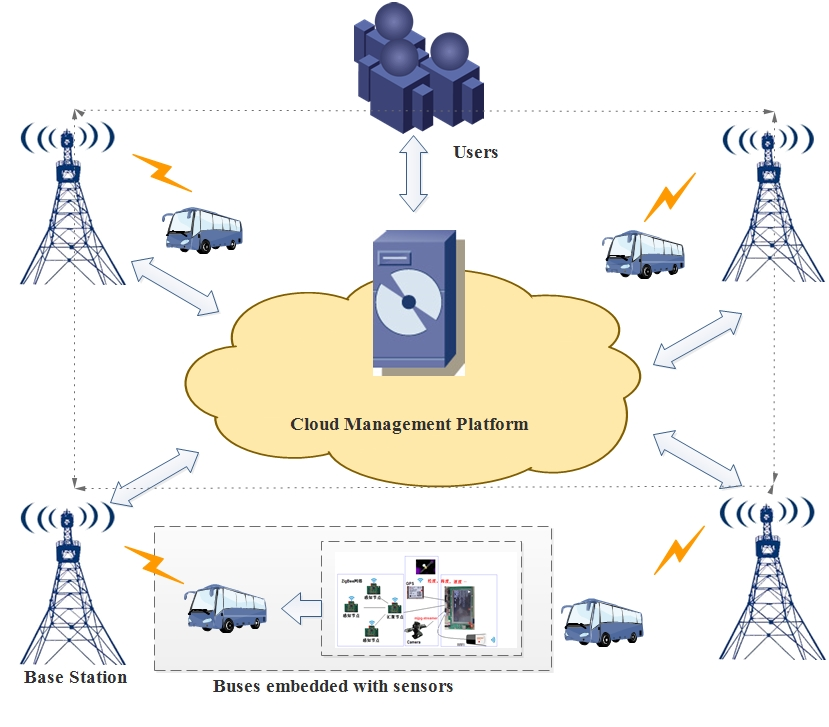
\includegraphics[width=1.0\linewidth]{Figure1.png}
	\caption[Fig.1]{An example of vehicle-based crowd sensing application.}
	\label{Figure1}
\end{figure}

In this paper, we investigate how to achieve a high quality of crowd-sensing with the predictable trajectory of PTs and the limited budget of CMP. Analying the relationship between STC and the predictable trajectory of PTs, we design a novel system model by considering the current and future trajectory of PTs and propose an algorithm to select PTs to carry out crowd-sensing tasks. Therefore, a high quality of crowd-sensing can be guaranteed for a period of time. Futhermore, we prove the selection of PTs problem is NP-hard and prove the proposed algorithm can achive a performance guarantee  no less than $\left ( 1-e^{-1} \right )$.

This paper is organized as follows. Section II reviews the related work. Section III introduces the system model and formulates the selection of PTs as an optimization problem. In Section IV we propose a novel algorithm to solve the selection problem of PTs and analyse the performance guarantee of this algorithm. Performance evaluation and analysis are provided in Section V. Finally, Section VI draws the conslusions of this paper.
\section{RELATED WORK}
In recent years, mobile crowd-sensing is a significant source of information for smart city. Many researchers are dedicated to study the vehicular application of crowd-sensing, e.g., traffic accident evidence collection [14]-[15], city block monitoring [16], bike-net for cyclist experience mapping [17], and many architectures of crowd-sensing. Authors of [11], [18]-[20] proposed a participants recruitment system and formulated the recruitment of participants as a constrained coverage problem but ignored the mobility of vehicle. Authors in [16] constructed a surveillance system based on vehicle with constraint network bandwidth. In [18], Gerla M et al. introduced a crowd-sensing service based on vehicle embedded with cameras to deliver images on demand to users. In [21], K.Han et al. proposed an incentive mechanisms for participant recruitment who interacted with a task requestor in a random order for maximizing the values of finished task. Authors of [22]-[23] studied location-based crowd-sensing systems and major concerned both spatial and temporal coverage based on current location of participants. However,  these crowd-sensing systems assumed that the initiators were capable to select participants as many as possible to conduct tasks and the trajectory of vehicles were known hypothetically, which is more suitable for the cases that there were a small number of participants,  the unlimited budget of initiators and the participants are unmovable. Distinguish from the problems above, we make an advance forward. To obtain a high quality of crowd-sensing, we not only consider the current and future trajectory of candidate, but also highlight the limited budget. Then we establish a novel system model and formulate the selection of PTs as an optimization issue solved by a performance guarantee approximation algorithm.
\section{SYSTEM MODEL AND PROBLEM FORMULATION}
\subsection{System Model }
 We divide a region $R$ into a serial of small segments. Let $R$ denotes the set of small segments, $R=\left \{ r_{1},r_{2},r_{3},...,r_{k} \right \}$. The CMP broadcasts a crowd-sensing task to be carried for a period of time, i.e. $T$. We assume the time is discrete, and we can get $T=\left \{ t_{1},t_{2},t_{3},...,t_{m} \right \}$. The PTs equips with sensor module that we have designed in [23]. Assume there are $n$ PTs can conduct sensing tasks and the set of PTs is denoted by $V=\left \{ v_{1},v_{2},v_{3},...,v_{n}\right \}$. Initially, the CMP obtains the current trajectroy of all PTs according to the schedule and broadcasts the data packet until receives the ACK. If the prediction is not consistent with the actual current trajectory obtained by Global Positioning System (GPS) [24] employed in PTs, it will be updated, respectively. Then we can get the trajectory of a PTs $v_{i}$ at a specific time  $t_{j}$, which is denoted by  $l_{i}(t_{j})\in R$. Thus the trajectory matrix of PTs can be represented as follows:
\setcounter{equation}{0}
\begin{equation}
L(V)=\begin{bmatrix}
l_{1}(t_{1})&l_{1}(t_{2})&... & l_{1}(t_{m})\\ 
l_{2}(t_{1})&l_{2}(t_{2})&... & l_{2}(t_{m})\\
.&. &.&.\\ 
.&. &.&.\\
.&. &.&.\\
l_{n}(t_{1})&l_{n}(t_{2})&... & l_{n}(t_{m})\\
\end{bmatrix}
\end{equation}
where the size of $L(V)$ is $n\times m$.


In practice, beacause nearby PTs usually upload similar information, we do not anticipate that all PTs are involved in crowd-sensing. In order to limit the number of PTs, we assume PTs need to be paid a sensing reward from CMP [9]-[11] . Next, we define the sensing reward.

\noindent
\textbf{Definition 1: Sensing Reward (SR)} a PT is selected to sense often associates with a reward. Let $c_{i}$ denotes the reward to $v_{i}$, which can be acquired through online bidding [30]. The reward vector $C$ is:
\begin{equation}
C=\left \{c_{1},c_{2},...,c_{n} \right \}
\end{equation}

With the limited budget of CMP, not all PTs participate in crowd-sensing. We adopt an indication vector $\Phi $ to imply whether a vehicle $v_{i}$ is selected or not,
\begin{equation}
\Phi_{i}= \left\{\begin{matrix}
1&v_{i}\in \Omega \\ 
0&otherwise\end{matrix}\right.
\end{equation}
where $\Omega \subseteq V$ is the set of selected PTs. Let $C(\Omega)$ denotes the total reward to PTs in $\Omega$, which can be computed as:
\begin{equation}
C(\Omega )=\left [ C,\Phi  \right ]
\end{equation}

As mentioned above, the quality of crowd-sensing is related to STC. Next, we will introduce the notion of spatial-temporal coverage.

\noindent
\textbf{Definition 2: Spatial-temporal Coverage (STC)} determines the quality of crowd-sensing. Formally, it can be defined as:
\begin{equation}
\textbf{STC}=\sum_{t_{j}\in T}\bigcup_{v_{i}\in \Omega}\left (l_{i}(t_{j}) \right)
\end{equation}

 In [23], we have designed a specific hardware system, which can collect various information such as temprature, flow of traffic, longitude, latitude, and so on. Based on the hardware system, we show an example to explain the implication of STC. In Fig. 2, if users request to collect the flow of traffic at region $R$ where is divided into a serial of segments, that is $R=$\{AB, AD, BC, BE, DE, EF, EH, DH, CF\}. The scheduled trajectory of \{Bus1, Bus2, Bus3, Bus4\} is \{BC, AB, AD, DE \}, \{BC, BE, EH \}, \{EH, HD, AD, AB, BE \}, \{EF, BE, AB, AD, DH \}, respectively. In a period of time \{$t_{1},t_{2},t_{3},t_{4}$\}  the trajectory of  Bus1 to Bus4 is \{BC, AD, DE, BC\}, \{BC, BE, BC, BE \},\{EH, HD, AB, BE\}, \{AB, BE, AD, DH\}, respectively. From equality $(1)$, we get:
\begin{equation}
L(V)=\begin{bmatrix}
BC &AD &DE &BC \\ 
BC& BE &BC &BE\\ 
AB& BE &AB &BE\\ 
AB& BE &AD &DH
\end{bmatrix}
\end{equation}

If the CMP is capable of selecting two PTs to sense, then we consider two cases as bellows:
\begin{equation}
\begin{aligned}
STC({Bus1,Bus2})=& \underset{t_{1}}{\underbrace{BC}}+\underset{t_{2}}{\underbrace{AD+BE}}+\underset{t_{3}}{\underbrace{DE+BC}}\\&+\underset{t_{4}}{\underbrace{BC+BE}}
\end{aligned}
\end{equation}
\begin{equation}
STC({Bus3,Bus4})= \underset{t_{1}}{\underbrace{AB}}+\underset{t_{2}}{\underbrace{BE}}+\underset{t_{3}}{\underbrace{AB+AD}}+\underset{t_{4}}{\underbrace{BE}}
\end{equation}

It can be seen that the set of \{Bus1, Bus2\} covers five different places in space and the segment of \{BC\} is covered three times, so the total STC is 7. On the contrary, the set of \{Bus3, Bus4\} only covers four different segements in space and the total STC is 5. So we are more willing to select \{Bus1, Bus2\} to sense.
\begin{figure}[t]
	\centering
	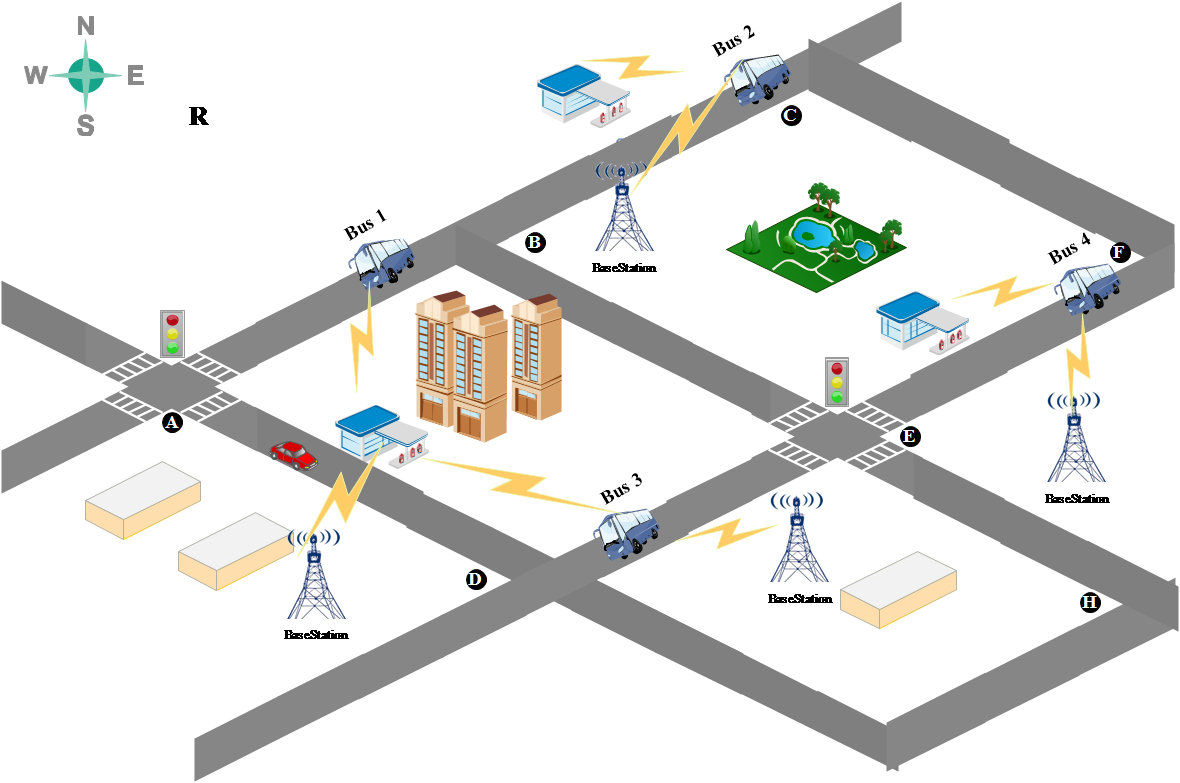
\includegraphics[width=1\linewidth]{Fig2(2).png}
	\caption{An example explains the notion of spatial-temporal Coverage.}
	\label{fig:figure4}
\end{figure}	

\subsection{Problem Statement} 
 Based on the system model, we are ready to formalize the selection of PTs as a optimization problem for maximizing the STC with limited budget.	


\noindent
\textbf{Definition 3: Selection of PTs Problem (SPTs)} is to determine a set of vehicle under the budget constraint $C_{max}$ with the objective of maximizing the spatial-temporal coverage.
\begin{equation}
\begin{matrix}
\textbf{max} \ STC(\Omega )\\\quad\quad\
\textbf{s.t.}\quad C(\Omega)\leqslant C_{max}\end{matrix}
\end{equation}

Actually, the data may have varying importance degrees at different segments and time, such as we are more interested in hotspot with high traffic flow. Therefore, we introduce priority power to indicate a public transport with a higher priority which is more likely to be selected to join crowd-sensing. Analyzing historical data, it is easy to acquire traffic performance index (TPI) [25] which is the congestion level of each segment. Let $D_{t_{j}}^{l_{i}}$ denotes the TPI of $l_{i} (t_{j})$ at a specific time $t_{j}$, and it is known and normalized between 0 and 1, e.g., $D_{t_{j}}^{l_{i}}\in (0,1]$. With the TPI we define priority power as follows:

\noindent
\textbf{Definition 4: Priority Power (PP)} is the priority of a vehicle to be selected to sense, which is a function of  $D_{t_{j}}^{l_{i}}$ defined as $W_{t_{j}}^{l_{i}}(D_{t_{j}}^{l_{i}})$. So $D_{t_{j}}^{l_{i}}\propto W_{t_{j}}^{l_{i}}$, thus the first order derivative of $W_{t_{j}}^{l_{i}}(D_{t_{j}}^{l_{i}})$ satisfies:
\begin{equation}
\frac{\mathrm{d}W_{t_{j}}^{l_{i}} }{\mathrm{d}D_{t_{j}}^{l_{i}}}> 0
\end{equation}
Therefore, priority power is expressed as:
\begin{equation}
W_{t_{j}}^{l_{i}}=\log_{2}(1+D_{t_{j}}^{l_{i}})
\end{equation}
With the priority power, the STC can be redefined as:
\begin{equation}
\sigma (\Omega )=\sum_{t_{j}\in T}\bigcup_{v_{i}\in \Omega }(l_{i}(t_{j})\cdot W_{t_{j}}^{l_{i}})
\end{equation}
and the SPTs can be rewritten as:
\begin{equation}
\begin{matrix}
\textbf{max}\  \sigma(\Omega)\\\quad\quad\quad\;\;\
\textbf{s.t.}\quad C(\Omega)\leqslant C_{max}\end{matrix}
\end{equation}

We hope that the solution of SPTs can be found with a time efficient. Unfortunately, it is NP-hard even though the trajectory of PTs are predictable. In the next section, we prove SPTs is NP-hard and propose an improved approximation algorithm based on greedy algorithm.
\section{SOLUTION TO THE SPTs}
\subsection{Complexity Analysis of SPTs}
\noindent
\textbf{Theorem 1.} The SPTs is NP-hard even though the trajectory of all vehicles are predictable.

\noindent
\textbf{Proof:} To prove the NP-hard hardness of SPTs, we should demonstrate it belongs to NP firstly. Assuming there is a possible solution $\Omega ^{'}$, it is clearly that the correctness of this solution can be certified in polynomial, the time complexity of the checking algorithm is O(n), which means SPTs is NP.

To prove SPTs is NP-hard further, we can construct a reduction in polynomial time from budgeted maximum coverage problem (MCP) as the known NP-hard [26] to SPTs. The MCP is defined as follows. 

Given a collection of sets $S=\left \{ S_{1},S_{2},.....,S_{n} \right \}$, each set $S_{i}$ with a cost  $c_{i},1\leqslant i\leqslant n$ takes values from $X=\left \{ x_{1},x_{2},.....,x_{m} \right \} $ associated with weights $w_{i},1\leqslant i\leqslant n$. The problem is to find a set $S^{'}\subseteq S$ satisfied the total cost and does not exceed a budget B.Then the total weight of $S^{'}$ is maximum simultaneously.
With all necessary conditions of SPTs, we make a mapping between MCP and SPTs as follows:
\begin{center}
$x_{i}\overset{mapping}{\rightarrow}l_{i}(t_{j})$,
$S_{i}\overset{mapping}{\rightarrow}L({\Omega ^{'}})$	
\end{center}
\begin{center}
$c_{i}\overset{mapping}{\rightarrow}C({\Omega ^{'}})$,
$B\overset{mapping}{\rightarrow}C_{max}$
\end{center}
where $\Omega ^{'}\subseteq V$. Eeach vehicle has a priority power which can be mapped to  $w_{i}$. We have reduced the decision version of MCP to the problem formulation of SPTs successfully. So we can obtain a corresponding instance from SPTs for any instance in MCP. As a result, the SPTs is NP-hard.

Consequently, to achieve a truthful and computationally efficient crowd-sensing, it is highly demanded to propose an approximate algorithm to solve SPTs.
\subsection{Approximate Algorithm to Solve SPTs}
We have analyzed the NP-hardness of SPTs, it becomes computationally impracticable to select an optimal set of PTs when the total number PTs is large. As for a metropolis like Beijing, the number of PTs under operations is about 30,000 per day by the end of 2016 [25]. To achieve a desired computational efficiency, we propose an approximate algorithm called efficient combination query algorithm (ECQA) to solve SPTs. The ECQA adopts a greedy strategy to solve SPTs. The greedy policy is to select one public transport with most reward efficiency, until the total SR exceeds the limited budget of CMP. Next we define the reward efficiency.

\noindent
\textbf{Definition 5: Reward Efficiency (RE)} indicates the marginal STC achieved per unit sensing reward. Mathematically, the RE can be computed as follows:
\begin{equation}
E_{i}=\frac{\sigma (\Omega ^{'})-\sigma (\Omega)}{c_{i}}
\end{equation}

The algorithm tries many rounds. A public transport with maximum RE is selected in each round. In equation (14), where $E_{i}$  denotes the reward efficient of vehicle $v_{i}$, $\Omega$ is solution obtained from $V$,  $\Omega ^{'}=\left \{ \Omega\cup v_{i}  \right \}$ and $v_{i}\in V-\Omega $. The algorithm will terminate until exceed the limited budget of CMP. The pseudo-code is listed in table 1.

\floatname{algorithm}{The pseudo-code of ECQA}
\renewcommand{\algorithmicrequire}{\textbf{Input:}}
\renewcommand{\algorithmicensure}{\textbf{Output:}}
\begin{algorithm}
	\caption{}	
	\begin{algorithmic}
		\Require set $V=\left \{  v_{1},v_{2},v_{3},...,v_{n}\right \}$ is PTs under operation, set $C=\left \{  c_{1},c_{2},c_{3},...,c_{n}\right \}$ is sensing reward to PTs, $C_{max}$ the limited budget of CMP, an initial set $S^{0}$ of cardinality is an integer as 3
		\Ensure set $\Omega $ is the best set of PTs selected by ECQA. 
		\State $max \gets 0$
		\State $\Omega \gets \varnothing$
		\State $S \gets \varnothing$
		\For{$S^{0}\subseteq V,C(S^{0})\leqslant C_{max}$}
			\State $S \gets S^{0}$
			\For{$v_{i}\in V-S$}
				\State $S^{'} \gets \left \{ S\cup v_{i} \right \}$
				\State $E_{i} \gets \frac{\sigma(S^{'})-\sigma (S)}{c_{i}}$
				\If{$E_{i}>max\quad \textbf{and}\quad C(S^{'})<C_{max}$}
					\State $S \gets S^{'}$
					\State $max \gets E_{i}$
				\EndIf
				\If{$\sigma(S)>\sigma()\Omega)$}
					\State $ \sigma \gets S$
				\EndIf
			\EndFor		
		\EndFor				
	\end{algorithmic}
\end{algorithm}


The ECQA has a performance guarantee $ \rho \leqslant 1$, which indicates we can obtain a solution is $\rho$ times of optimal solution in NP-hard problem [26]. In this paper, the ECQA can achieve a lower bound ratio of  $\left (1-e^{-1}  \right )$ when the cardinality as $q$ of set $S^{0}$ is no less than three, i.e.,  $q\geqslant 3$. Next, we prove the following theorem about the performance guarantee of ECQA.

\noindent
\textbf{Theorem 2.} The ECQA can achieve a worst performance guarantee to be  $\left (1-e^{-1}  \right )$ of optimum solution when $\left |q\geqslant 3 \right|$. 
\begin{equation}
\sigma (\Omega )\geqslant \left (1-e^{-1}  \right )\cdot \sigma (Opt), q\geqslant 3
\end{equation}
where $Opt$ is optimum solution.

\noindent
\textbf{Proof:} Let's redefine $v_{i}\in V,i=1,2,3,...,r$ as a public transport added into $\Omega$ in i-th iteration, Let $\Omega_{k}$ denote $ \bigcup_{i=1}^{k}v_{i}$, and $\Omega =\Omega _{r}$. To prove inequality (15), the following two inequalities we can derive from [27], After $i-th$, $ i=1,2,3,...,r+1$ iterations, we can get:
\begin{equation}
\sigma (\Omega _{i})\geqslant \left [ 1-\coprod_{m=1}^{i}(1-\frac{c_{m}}{C_{max}}) \right ]\cdot \sigma (Opt)
\end{equation}
\begin{equation}
\begin{aligned}
\sigma (\Omega _{r+1})&\geqslant \left [ 1-\coprod_{m=1}^{r+1}(1-\frac{c_{m}}{C_{max}}) \right ]\cdot \sigma (Opt) \\ & \geqslant \left [ 1-\left ( 1-\frac{1}{r+1} \right )^{r+1} \right ]\cdot\sigma (Opt)\\&\geqslant \left (1-e^{-1}  \right )\cdot\sigma (Opt) 
\end{aligned}
\end{equation}
where $c_{m}$ denotes the sensing reward to $v_{m}$. The detailed proof of inequalities (16), (17) can be found in [26]-[27]. We can easily know that (17) is equivalent to following inequality:
\begin{equation}
\begin{aligned}
\sigma (\Omega _{r+1})=\sigma(\Omega _{r})+\sigma(\left \{ v_{r+1}\right \})\geqslant\left ( 1-e^{-1} \right ) \cdot \sigma (Opt)
\end{aligned}
\end{equation}
where $v_{r+1}$ is selected at $r+1$ round but not added to $\Omega$ because it exceeds the limited budget $C_{max}$. Applying (16) to (18), we get:
\begin{equation}
\sigma (\Omega _{r}-S^{0})+\sigma (\left \{ v_{r+1} \right \})\geqslant \left ( 1-e^{-1} \right )\cdot \sigma (Opt-S^{0})
\end{equation}
where $Opt-S^{0}$ means that an element belongs to set $Opt$ but not in $S^{0}$.

Assuming $\sigma\left(\left \{ v_{r+1} \right \}\right)$ is greater than $\sigma\left ( \left \{ v_{i} \right \} \right)$, $i=1,2,3,...,r$, $v_{r+1}$ should be selected before $v_{i}$ and included in $\Omega _{r}$, the opposite is true. Therefore, we can get:
\begin{equation}
q\cdot \sigma \left ( \left \{ v_{r+1} \right \} \right )\leqslant \sigma \left ( S^{0} \right )
\end{equation}
From (19), (20) the following inequality can be hold
\begin{equation}
\sigma \left ( \Omega _{r} \right )\geqslant \left ( 1-e^{-1} \right )\cdot \sigma (Opt-S^{0})+(1-q^{-1})\cdot \sigma (S^{0})
\end{equation}
where $e$ is less than three, hence
\begin{equation}
\sigma \left ( \Omega _{r} \right )\geqslant \left ( 1-e^{-1} \right )\cdot (\sigma (Opt-S^{0})+\sigma (S^{0}))
\end{equation}
if and only if $q\geqslant 3$, the inequality (21) holds. Clearly, $\sigma(Opt-S^{0})+\sigma (S^{0})=\sigma (Opt)$, and then
\begin{equation}
\sigma(\Omega_{r})\geqslant (1-e^{-1})\cdot \sigma(Opt), \ for \ q\geqslant 3
\end{equation}
proves the theorem.


\section{VALIDATION}
Extensive simulations have been conducted to evaluate the performance of our proposed algorithm. The traffic trace dataset we used, the simulation setup, the compared algorithms, and the performance comparison and discussion are presented as follows.


\subsection{Real Traffic Track Used and Simulation Setup}
In our simulation, we adopt the T-Drive trajectory dataset [28]-[29] which contains a one-week trajectory of 10,357 buses. The dataset contains information about identification, arrival time, longitude, latitude, such as [ id: 10002, arival time: 2008-02-03 10:06:48, longitude: 116.41904, latitude: 39.93963 ]. The total trajectory of buses in this dataset is about 15 million and the total distance of the trajectory reaches 9 million kilometers. We import the data into the Google Global Mapper. As shown in Fig.3, the distribution of the trajectory of vehicles can cover the whole traffic network of Beijing. We extract a subset of buses from the whole dataset for performance research, and the trajectory of the subset spans from February 3, 2008, 6 AM to 10 PM. In our simulation, the size of region is $6km\times 6km$, which is divided into 36 squares with a width of $1km$. The period of time is from $1min$ to $15min$, PTs are associated with SR, which is uniformly distributed in $[0.7, 1.2]$ and the limited budget $C_{max}$ is $[3, 10]$. 
\begin{figure}
	\centering
	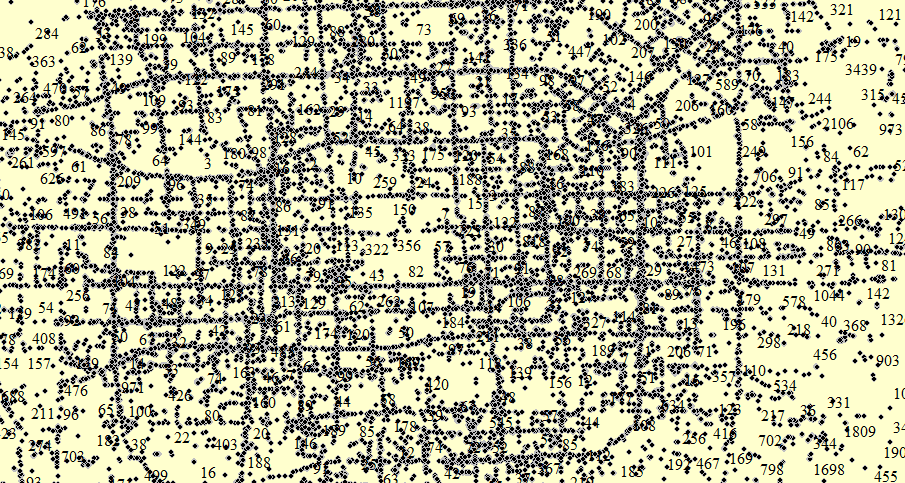
\includegraphics[width=0.85\linewidth]{fig3-1.png}
	\caption{The vehicle trajectory distribution in Beijing Metropolis according to the dataset}
	\label{fig:figure4}
\end{figure} 

\subsection{Algorithm in Comparison}
The quality of crowd-sensing is related to STC, we evaluate how the total sensing reward $C_{max}$, the number of time period $m$, and the initial size of solution $q$ affect the performance. In this paper, we compare our algorithm with two algorithms and use unpredictable trajectory to vertify the better performance of it. 1) The enumerative algorithm (EA) can always select a optimum set of PTs by exhaustive search. However, the SPTs is NP-hard, when the number of PTs is larger, it becomes infeasible to obtain the optimal solution in polynomial time. Thus, the EA is applied simply when the number of PTs is small. 2) The simulated annealing algorithm (SAA) is often used to solve optimization problems, we improve a SAA to compute the SPTs for maximizing the STC. 3) Using unpredictable trajectory means that we only take the current trajectory of PTs into account as [19]. Furthermore, the results are also compared with the lower bound performance guarantee STC $EA\cdot(1-e^{-1})$.

\begin{figure}[h]
	\centering
	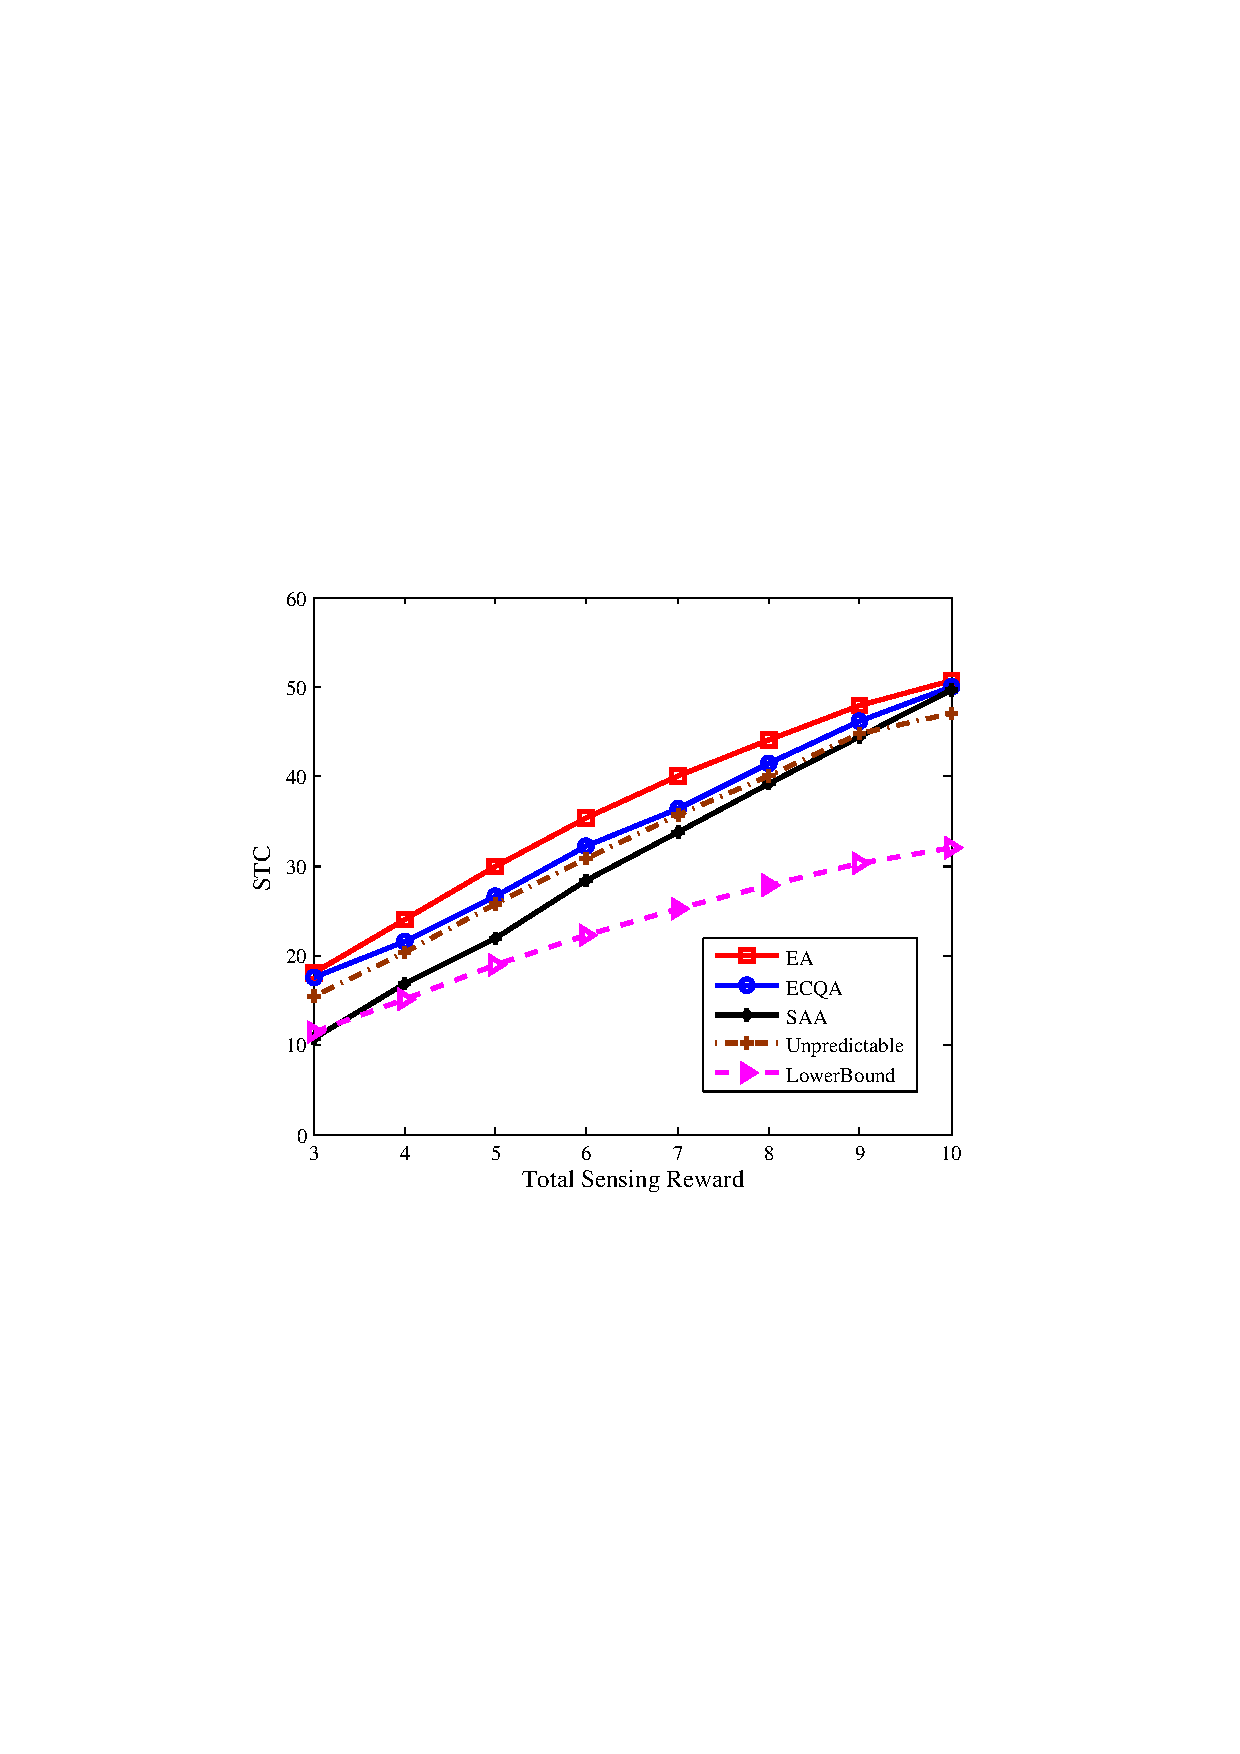
\includegraphics[width=0.85\linewidth]{figure4.pdf}
	\caption{The total sensing reward $C_{max}$ is [3,10], the initial size of solution is 3, the number of period time is 6.}
	\label{fig:figure4}
\end{figure}

\begin{figure}[h]
	\centering
	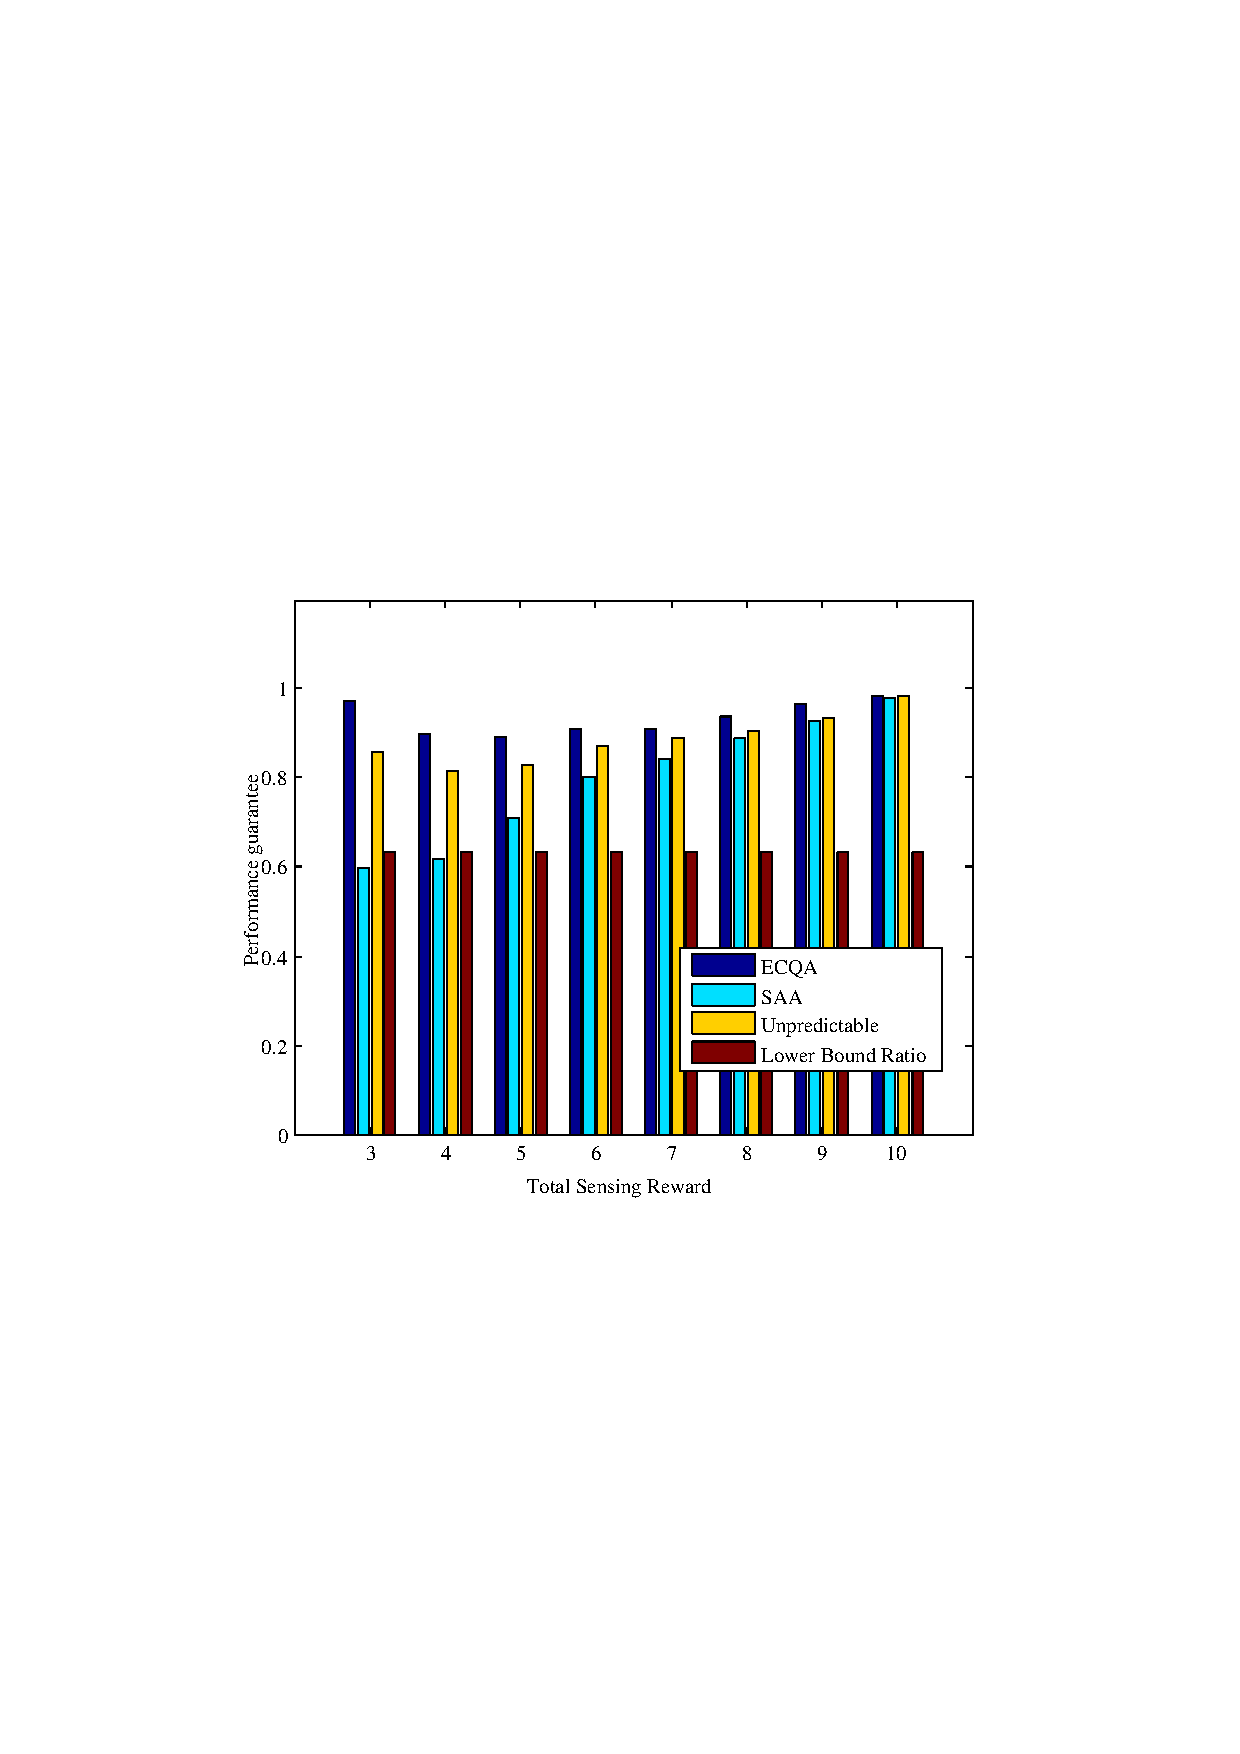
\includegraphics[width=0.85\linewidth]{figure7.pdf}
	\caption{The total sensing reward $C_{max}$ is [3,10], the initial size of solution is 3, the number of period time is 6.}
	\label{fig:figure5}
\end{figure}

\begin{figure}
	\centering
	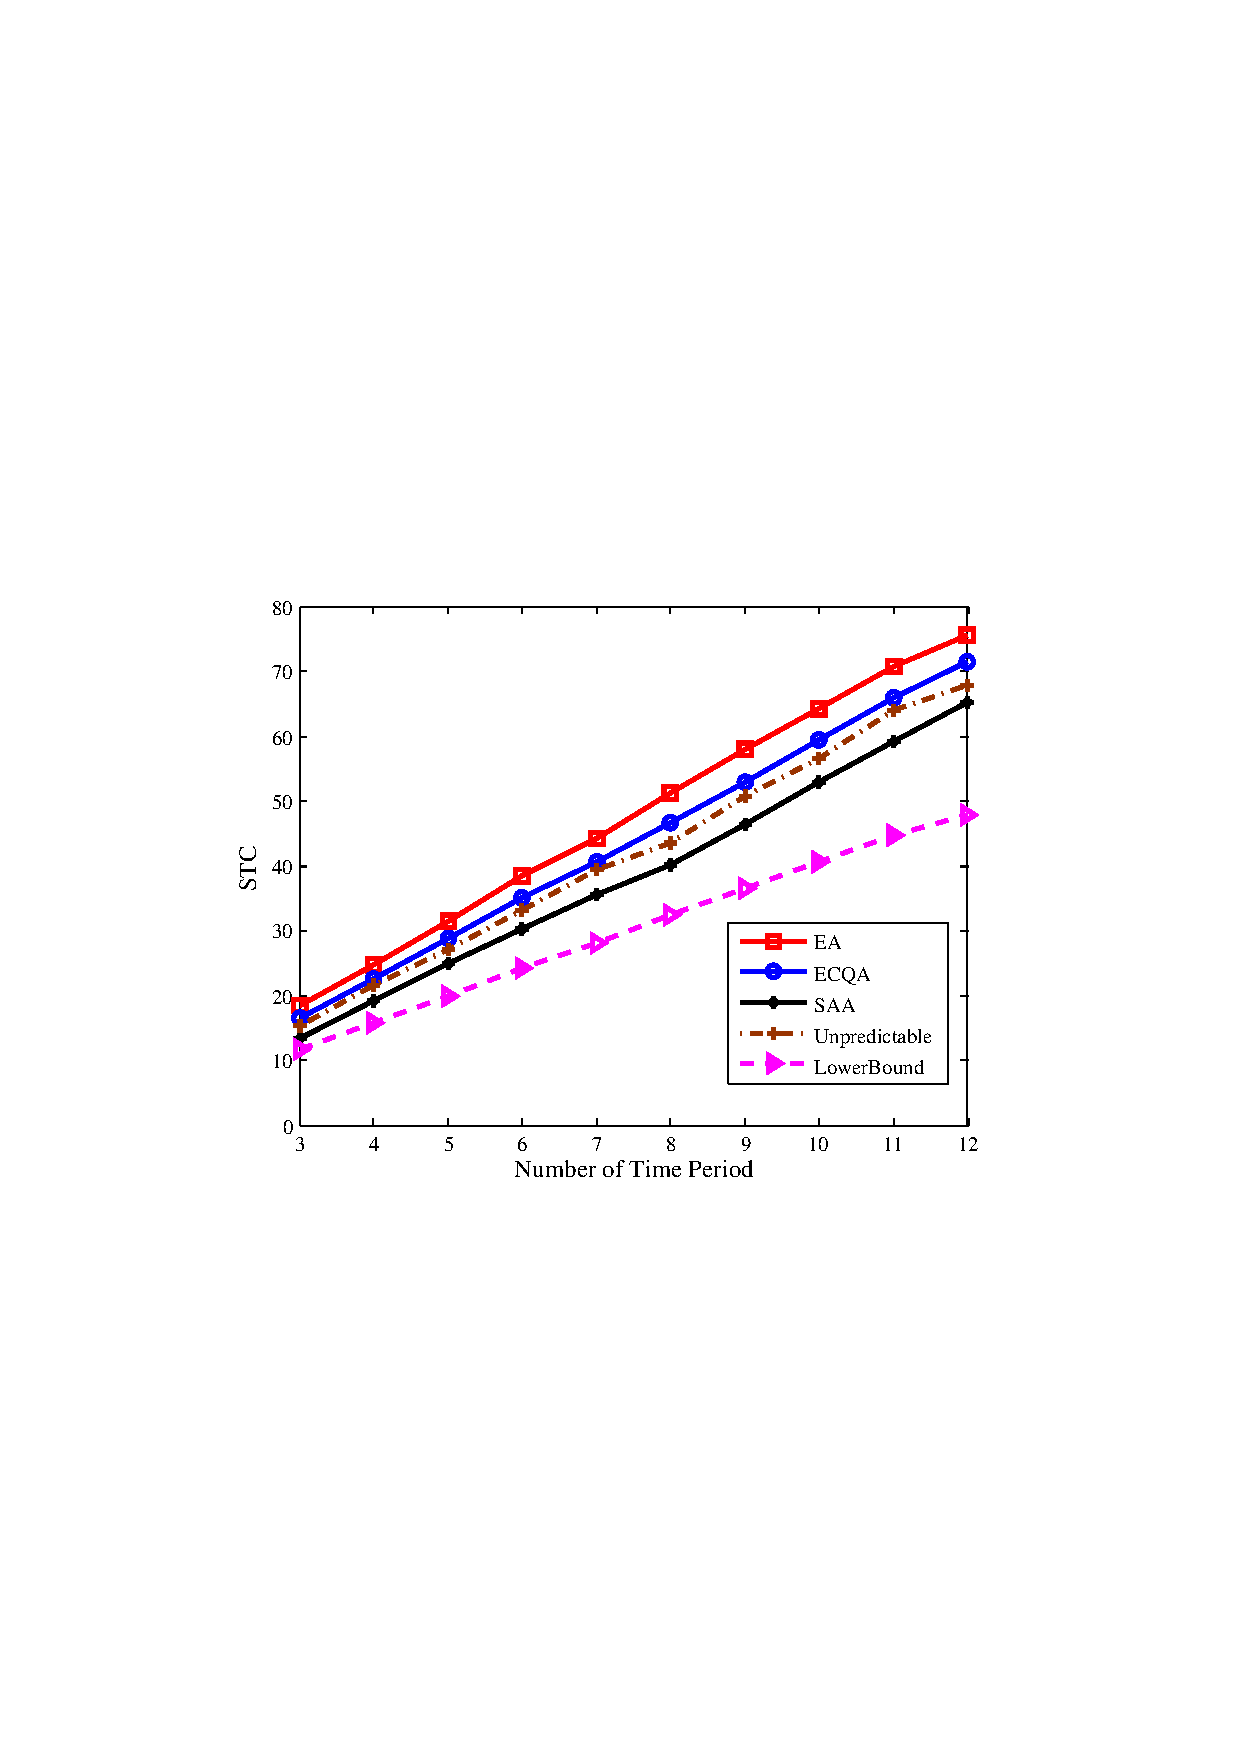
\includegraphics[width=0.85\linewidth]{figure5.pdf}
	\caption{ The number of period is [3, 12], the total sensing reward $C_{max}$ is 6, the initial size of solution is 3.}
	\label{fig:figure6}
\end{figure}


\begin{figure}[h]
	\centering
	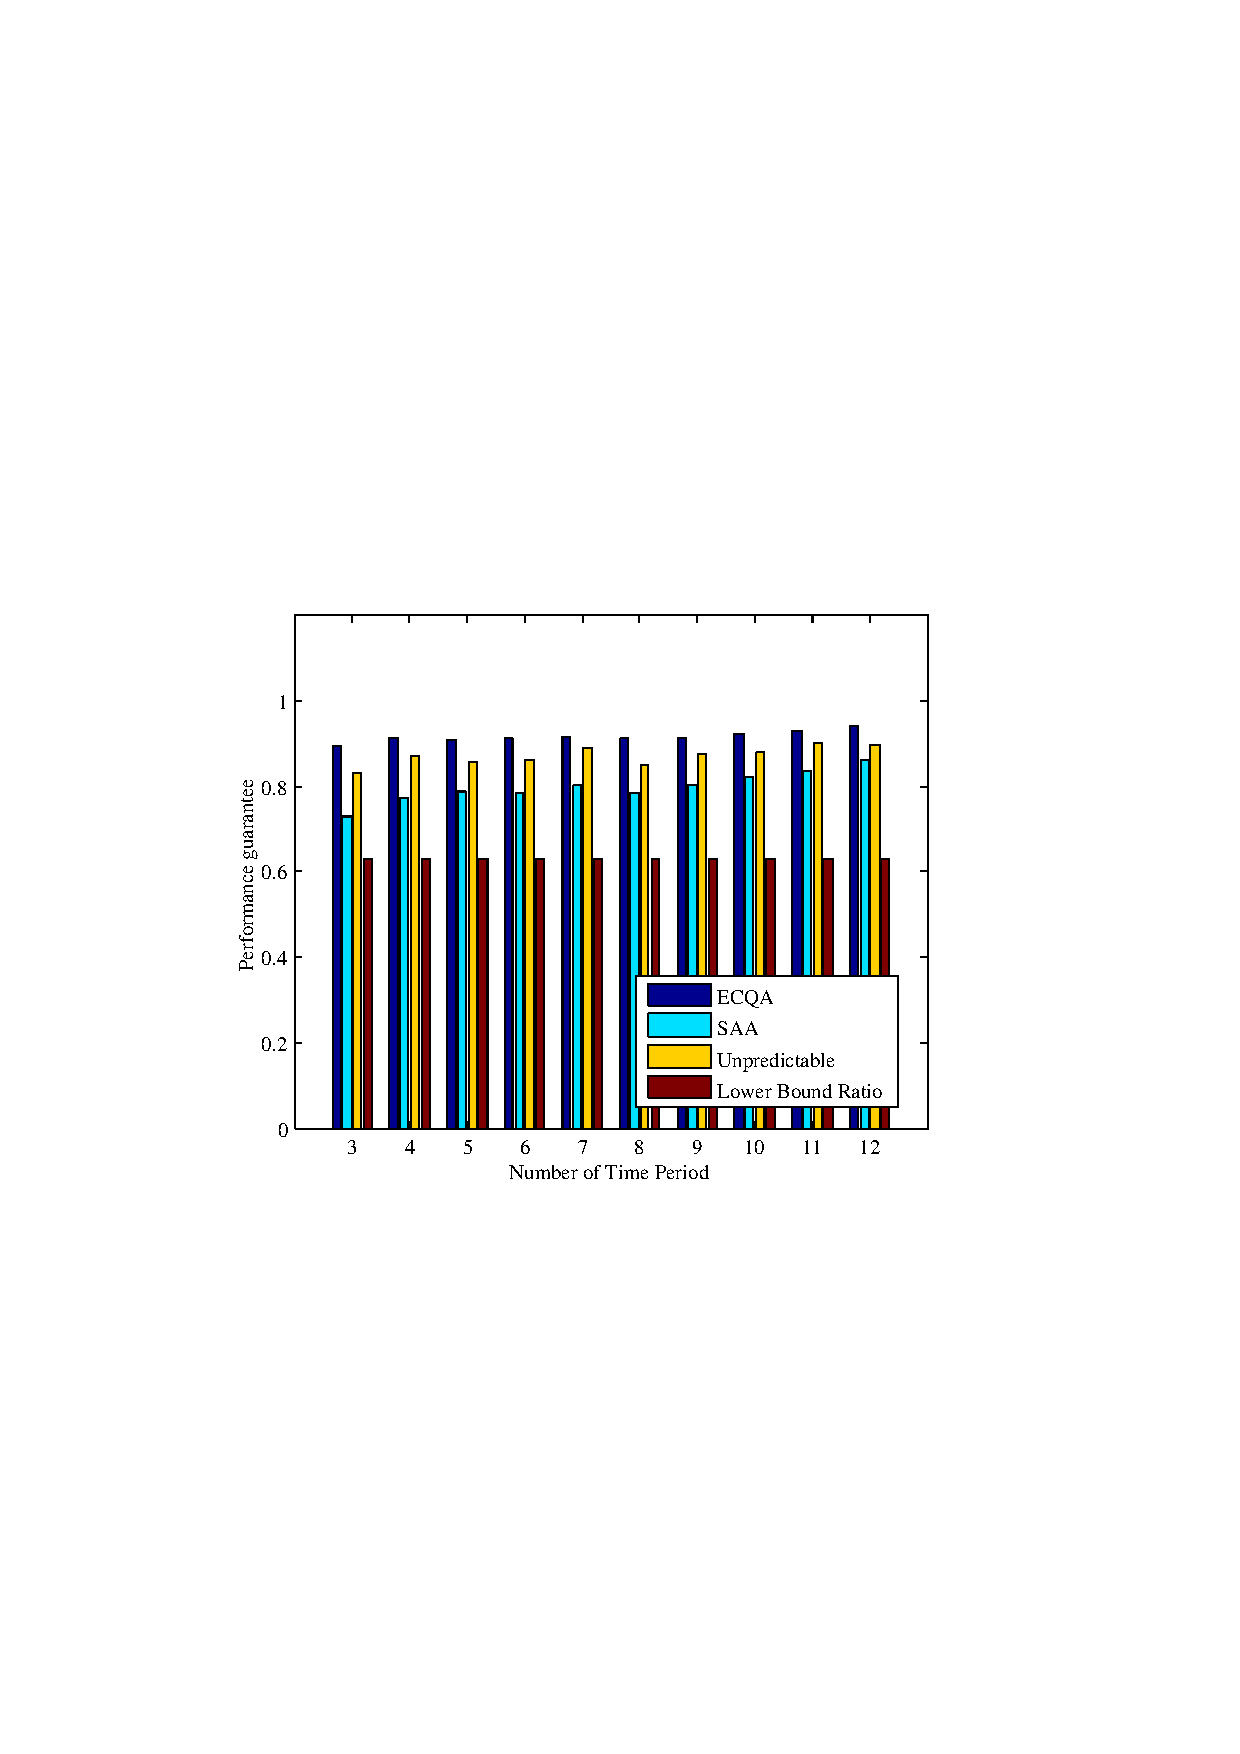
\includegraphics[width=0.81\linewidth]{figure8.pdf}
	\caption{The number of period is [3, 12], the total sensing reward $C_{max}$ is 6, the initial size of solution is 3.}
	\label{fig:figure7}
\end{figure}
\begin{figure}[h]
	\centering
	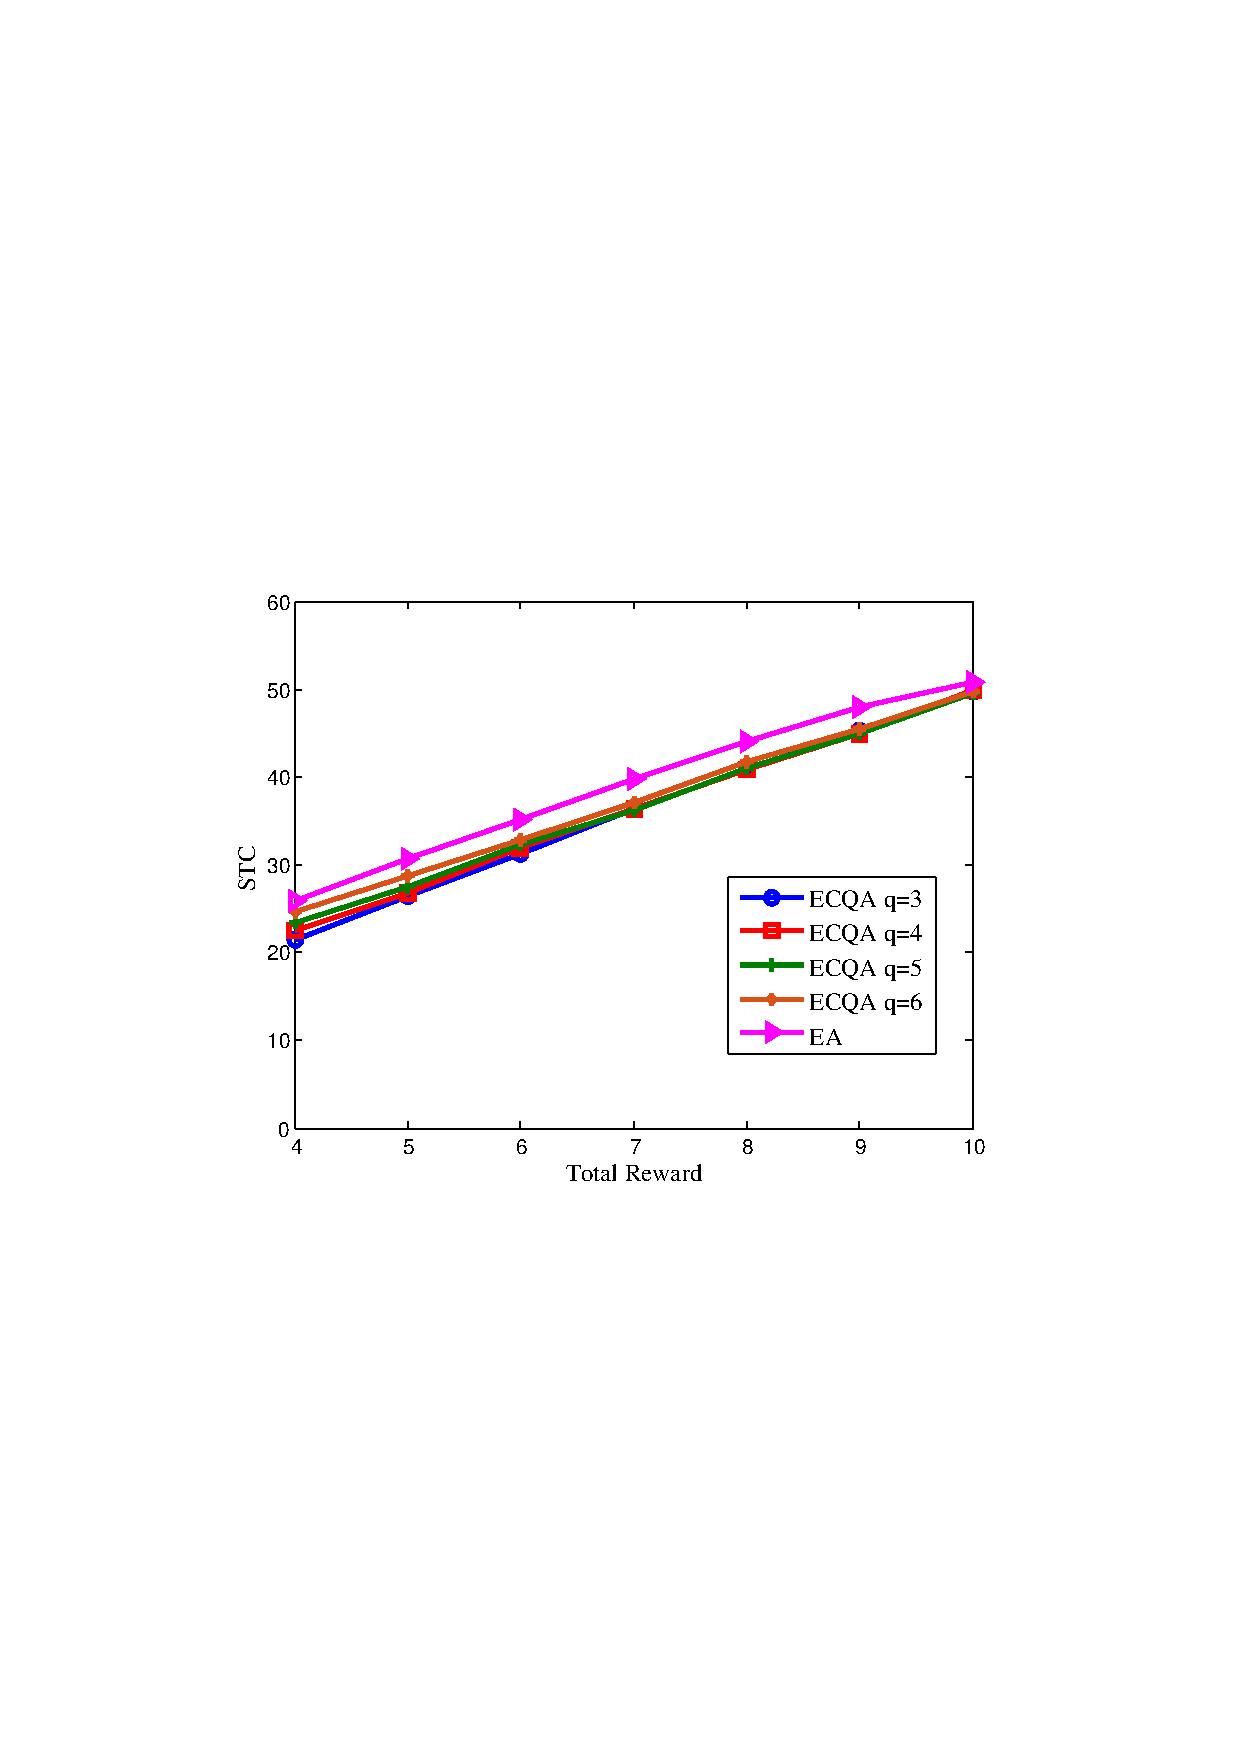
\includegraphics[width=0.85\linewidth]{figure6.pdf}
	\caption{The initial size of solution is [3, 6], the total sensing reward is [4, 10], the number of period time is 6.}
	\label{fig:figure8}
\end{figure}

\begin{figure}[h]
	\centering
	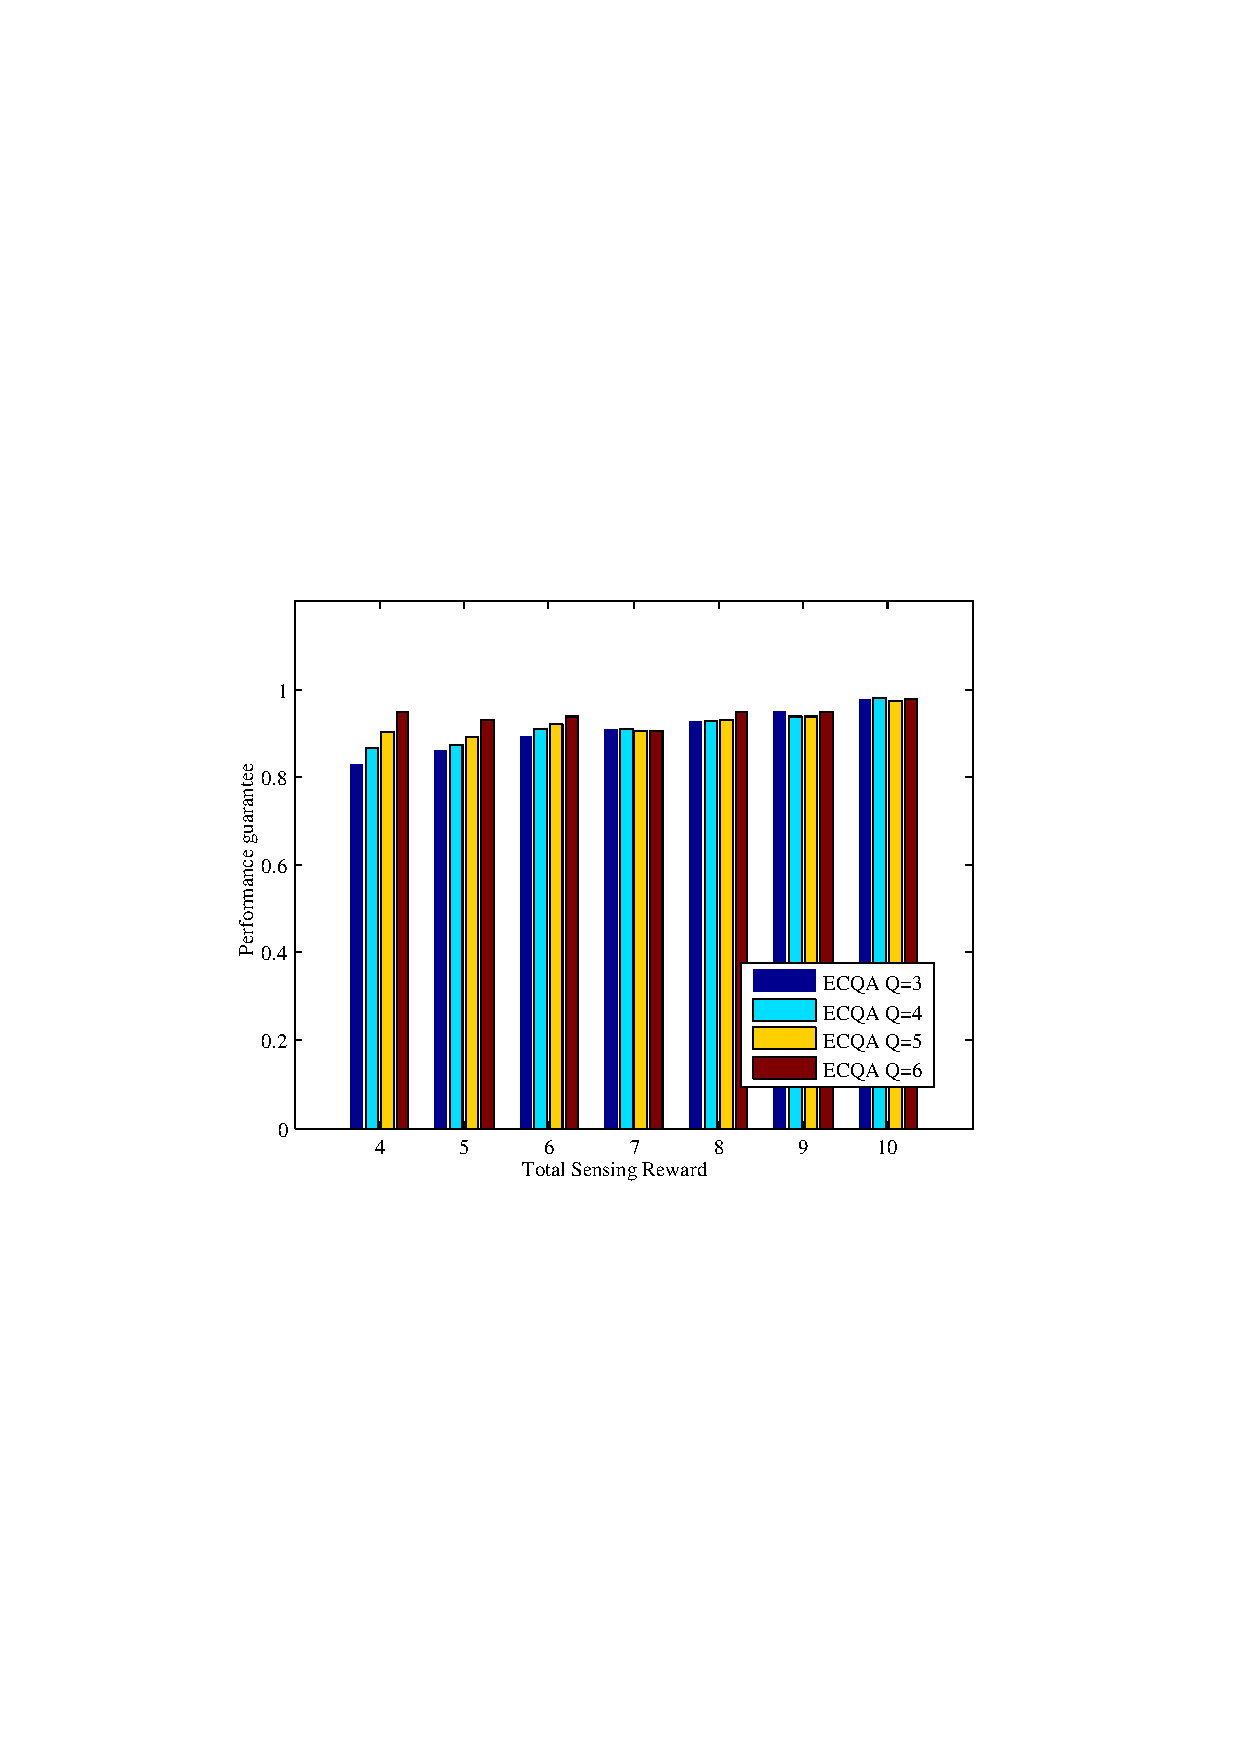
\includegraphics[width=0.85\linewidth]{figure9.pdf}
	\caption{The initial size of solution is [3, 6], the total sensing reward is [4, 10], the number of period time is 6.}
	\label{fig:figure9}
\end{figure}

Fig. 4 to Fig. 9 illustrate the performance during the variation of the total sensing reward $C_{max}$, the number of period time $m$ and the initial size of solution $q$. In this group of simulations, we extract 10 vehicles from dataset. From Fig. 4 to Fig. 9, we can observe that the proposed algorithm in this paper outperforms the SAA, and gets closer to the optimal EA. In Fig. 4, the STC of our algorithm is larger than the SAA. And when the sensing reward is enough, the STC of ECQA and SAA tend to be the optimum. This is because the budget is enough, the CMP may select all PTs to carry out task, the result fits in with the reality. In Fig. 5, the performance guarantee of ECQA fluctuates around 0.9 and still provides a performance guarantee larger than $(1-e^{-1})\approx0.6321$ as we had proved. This result indicates that in real cases, our algorithm is more likely to achieve full-coverage with a high quality of crowd-sensing. Fig. 6 shows that along with the increase of the number of period time $m$, the STC of ECQA and alternative algorithms have been an rising trend. This is because one segment may be covered many times at difference period times. Additionally, the performance gap between ECQA and EA stayed nearly constant and the performance guarantee is greater than 0.9 consistently as Fig. 7 shown. In Fig. 8 and Fig. 9, we study the influence of the important parameter q on performance of ECQA, the $q$ is varied from 3 to 6. It is easy to see that, the total sensing reward is less than 7, the STC increases with $q$, otherwise is closer. This results can be understood since the total sensing reward is insufficient and the $q$ is larger. ECQA primarily searches a larger domain for optimal solution, but it takes longer execution time actually. In contract, $q$ has slightly impact on STC, which suggests that we can get a good performance even with a small $q$ and spend less running time simultaneously. From Fig. 4 to Fig. 7, we can observe the truth that the performance of proposed algorithm using unpredictable trajectory is better than SAA, LowerBound, and gets closer to ECQA. There is an underlying problem can not be ignored, i.e., when the system selects a best solution by using the proposed algorithm with unpredictable trajectory, the PTs covers the same segment at different sensing time, which means the best solution merely make sure the STC is continuous in time, but discrete in space.



\section{CONCLUTION}
In this paper, we have introduced crowd-sensing into vehicular network to construct a vehicle-based crowd-sensing network. The quality of crowd-sensing is sensitive to the trajectory of participants, so we took advantage of scheduled mobility pattern of PTs with predictable trajectory. In this scenario, we need to address how to select PTs to carry out sensing tasks for a high quality of crowd-sensing.
We have analyzed the relationship between STC and the predictable trajactory of PTs, and have designed a system model by cosidering the current and future trajectory. Then based on system model, we have formulated the selection of PTs as a optimization problem, which was proved as a NP-hard problem. In oder to maximize STC in polynomial time, we have proposed ECQA to achieve a performance guarantee closer to $1$. Finally, the simulations have been performed by using T-Drive trajectory dataset, the results have shown the ECQA outperforms other exsiting algorithms.







% You must have at least 2 lines in the paragraph with the drop letter
% (should never be an issue)








% An example of a floating figure using the graphicx package.
% Note that \label must occur AFTER (or within) \caption.
% For figures, \caption should occur after the \includegraphics.
% Note that IEEEtran v1.7 and later has special internal code that
% is designed to preserve the operation of \label within \caption
% even when the captionsoff option is in effect. However, because
% of issues like this, it may be the safest practice to put all your
% \label just after \caption rather than within \caption{}.
%
% Reminder: the "draftcls" or "draftclsnofoot", not "draft", class
% option should be used if it is desired that the figures are to be
% displayed while in draft mode.
%
%\begin{figure}[!t]
%\centering
%\includegraphics[width=2.5in]{myfigure}
% where an .eps filename suffix will be assumed under latex, 
% and a .pdf suffix will be assumed for pdflatex; or what has been declared
% via \DeclareGraphicsExtensions.
%\caption{Simulation results for the network.}
%\label{fig_sim}
%\end{figure}

% Note that the IEEE typically puts floats only at the top, even when this
% results in a large percentage of a column being occupied by floats.


% An example of a double column floating figure using two subfigures.
% (The subfig.sty package must be loaded for this to work.)
% The subfigure \label commands are set within each subfloat command,
% and the \label for the overall figure must come after \caption.
% \hfil is used as a separator to get equal spacing.
% Watch out that the combined width of all the subfigures on a 
% line do not exceed the text width or a line break will occur.
%
%\begin{figure*}[!t]
%\centering
%\subfloat[Case I]{\includegraphics[width=2.5in]{box}%
%\label{fig_first_case}}
%\hfil
%\subfloat[Case II]{\includegraphics[width=2.5in]{box}%
%\label{fig_second_case}}
%\caption{Simulation results for the network.}
%\label{fig_sim}
%\end{figure*}
%
% Note that often IEEE papers with subfigures do not employ subfigure
% captions (using the optional argument to \subfloat[]), but instead will
% reference/describe all of them (a), (b), etc., within the main caption.
% Be aware that for subfig.sty to generate the (a), (b), etc., subfigure
% labels, the optional argument to \subfloat must be present. If a
% subcaption is not desired, just leave its contents blank,
% e.g., \subfloat[].


% An example of a floating table. Note that, for IEEE style tables, the
% \caption command should come BEFORE the table and, given that table
% captions serve much like titles, are usually capitalized except for words
% such as a, an, and, as, at, but, by, for, in, nor, of, on, or, the, to
% and up, which are usually not capitalized unless they are the first or
% last word of the caption. Table text will default to \footnotesize as
% the IEEE normally uses this smaller font for tables.
% The \label must come after \caption as always.
%
%\begin{table}[!t]
%% increase table row spacing, adjust to taste
%\renewcommand{\arraystretch}{1.3}
% if using array.sty, it might be a good idea to tweak the value of
% \extrarowheight as needed to properly center the text within the cells
%\caption{An Example of a Table}
%\label{table_example}
%\centering
%% Some packages, such as MDW tools, offer better commands for making tables
%% than the plain LaTeX2e tabular which is used here.
%\begin{tabular}{|c||c|}
%\hline
%One & Two\\
%\hline
%Three & Four\\
%\hline
%\end{tabular}
%\end{table}


% Note that the IEEE does not put floats in the very first column
% - or typically anywhere on the first page for that matter. Also,
% in-text middle ("here") positioning is typically not used, but it
% is allowed and encouraged for Computer Society conferences (but
% not Computer Society journals). Most IEEE journals/conferences use
% top floats exclusively. 
% Note that, LaTeX2e, unlike IEEE journals/conferences, places
% footnotes above bottom floats. This can be corrected via the
% \fnbelowfloat command of the stfloats package.








% if have a single appendix:
%\appendix[Proof of the Zonklar Equations]
% or
%\appendix  % for no appendix heading
% do not use \section anymore after \appendix, only \section*
% is possibly needed

% use appendices with more than one appendix
% then use \section to start each appendix
% you must declare a \section before using any
% \subsection or using \label (\appendices by itself
% starts a section numbered zero.)
%


\appendices

%Appendix one text goes here.

%% you can choose not to have a title for an appendix
%% if you want by leaving the argument blank


% use section* for acknowledgment
%\section*{Acknowledgment}

\section*{Acknowledgment}


This paper was supported by the National Science Foundation of China, $NO.61271186$ and National Key R\&D Program of China, $NO.2017YFC0804404$, Beijing Municipal Commission of Education (The City's Vehicle Sensing Grid Construction Based on Public Transportation Network).
%The authors would like to thank...


% Can use something like this to put references on a page
% by themselves when using endfloat and the captionsoff option.
\ifCLASSOPTIONcaptionsoff
  \newpage
\fi



% trigger a \newpage just before the given reference
% number - used to balance the columns on the last page
% adjust value as needed - may need to be readjusted if
% the document is modified later
%\IEEEtriggeratref{8}
% The "triggered" command can be changed if desired:
%\IEEEtriggercmd{\enlargethispage{-5in}}

% references section

% can use a bibliography generated by BibTeX as a .bbl file
% BibTeX documentation can be easily obtained at:
% http://mirror.ctan.org/biblio/bibtex/contrib/doc/
% The IEEEtran BibTeX style support page is at:
% http://www.michaelshell.org/tex/ieeetran/bibtex/
%\bibliographystyle{IEEEtran}
% argument is your BibTeX string definitions and bibliography database(s)
%\bibliography{IEEEabrv,../bib/paper}
%
% <OR> manually copy in the resultant .bbl file
% set second argument of \begin to the number of references
% (used to reserve space for the reference number labels box)
\begin{thebibliography}{1}

\bibitem{IEEEhowto:kopka}
Zhu.Y, Bao.Y, Li.B, ``On Maximizing Delay-Constrained Coverage of Urban Vehicular Networks,'' \textit{IEEE Journal on Selected Areas in Communications}, 2012, 30(4): 804-817.

\bibitem{IEEEhowto:kopka}
Dejun Yang, Guoliang Xue, Xi Fang, and Jian Tang, ``Crowdsourcing to smart phones: incentive mechanism design for mobile phone sensing,''  \textit{ACM MOBICOM}, 2012. 

\bibitem{IEEEhowto:kopka}
Mohammad Nozari Zarmehri and Ana Aguiar, ``Supporting sensing application in vehicular networks,'' \textit{ACM CHANTS}, 2012.

\bibitem{IEEEhowto:kopka}
Koukoumidis, Emmanouil, L. S. Peh, and M. R. Martonosi. ``SignalGuru:leveraging mobile phones for collaborative traffic signal schedule advisory,'' \textit{International Conference on Mobile Systems, Applications, and Services DBLP}, 2011: 127-140.

\bibitem{IEEEhowto:kopka}
A. Thiagarajan et al . ``Vtrack: Accurate, energy-aware road traffic delay estimation using mobile phones,'' \textit{7th ACM Conf.Embedded Netw. Sensor Syst., ACM}, 2009, pp. 85–98.

\bibitem{IEEEhowto:kopka}
Dutta P, Aoki P M, Kumar N, et al. ``Common Sense:participatory urban sensing using a network of handheld air quality monitors,'' \textit{International Conference on Embedded Networked Sensor Systems}, 2009: 349-350.

\bibitem{IEEEhowto:kopka}
Farshad, Arsham, M. K. Marina, and F. Garcia. ``Urban WiFi characterization via mobile crowdsensing,'' \textit{Noms IEEE/IFIP Network Operations Management Symposium IEEE}, 2014: 1-9.

\bibitem{IEEEhowto:kopka}
Feng Z, Zhu Y, Zhang Q, et al. ``TRAC: Truthful auction for location-aware collaborative sensing in mobile crowdsourcing,'' \textit{INFOCOM 2014 Proceedings IEEE}, , 2014: 1231-1239.

\bibitem{IEEEhowto:kopka}
D. Yang, G. Xue, and et al.. ``Crowdsourcing to smartphones: Incentive mechanism design for mobile phone sensing,'' \textit{MobiCom 2012}, pp. 173–184.

\bibitem{IEEEhowto:kopka}
Reddy, Sasank, et al. ``Examining micro-payments for participatory sensing data collections,'' \textit{ACM International Conference on Ubiquitous Computing ACM}, 2010: 33-36.

\bibitem{IEEEhowto:kopka}
He, Zongjian, J. Cao, and X. Liu. ``High quality participant recruitment in vehicle-based crowdsourcing using predictable mobility,'' \textit{Computer Communications IEEE}, 2015: 2542-2550.

\bibitem{IEEEhowto:kopka}
Kazemi L, Shahabi C. ``GeoCrowd:enabling query answering with spatial crowdsourcing,'' \textit{International Conference on Advances in Geographic Information Systems}, 2012: 189-198.

\bibitem{IEEEhowto:kopka}
Huang, Jihua, and H. S. Tan. ``Vehicle future trajectory prediction with a DGPS/INS-based positioning system,'' \textit{American Control Conference IEEE}, 2006: 6 pp.

\bibitem{IEEEhowto:kopka}
Hussain R, Abbas F, Son J, et al. ``Vehicle Witnesses as a Service: Leveraging Vehicles as Witnesses on the Road in VANET Clouds,'' \textit{IEEE International Conference on Cloud Computing Technology and Science}, 2013: 439-444.

\bibitem{IEEEhowto:kopka}
Thiagarajan A, Ravindranath L, Lacurts K, et al. ``VTrack: accurate, energy-aware road traffic delay estimation using mobile phones,'' \textit{ACM Conference on Embedded Networked Sensor Systems}, 2009: 85-98.
 
\bibitem{IEEEhowto:kopka}
Lee J L, Kim D, Fan L, et al, ``Barrier-Coverage for City Block Monitoring in Bandwidth Sensitive Vehicular Adhoc Networks,'' \textit{International Conference on Mobile Ad-Hoc and Sensor Networks.} 2015: 80-87.

\bibitem{IEEEhowto:kopka}
Reddy S, Shilton K, Burke J, et al. ``Using Context Annotated Mobility Profiles to Recruit Data Collectors in Participatory Sensing,'' 2009, 5561: 52-69.
 
\bibitem{IEEEhowto:kopka}
Gerla M, Pau G, Weng J T. ``Pics-on-wheels: Photo surveillance in the vehicular cloud. International Conference on Computing,'' \textit{NETWORKING and Communications}, 2013: 1123-1127.
\bibitem{IEEEhowto:kopka}
Reddy, Sasank, D. Estrin, and M. Srivastava. ``Recruitment Framework for Participatory Sensing Data Collections,'' \textit{International Conference}, May 17-20, 2010. 2010: 138-155.
\bibitem{IEEEhowto:kopka}
X. Zhang, Z. Yang, Y. Liu, J. Li and Z. Ming. ``Toward efficient mechanisms for mobile crowdsensing.'' \textit{IEEETrans.Veh.Technol}, vol.66, no.2, pp. 1760–1771, Feb. 2017. 

\bibitem{IEEEhowto:kopka}
K. Han, C. Zhang, J. Luo, M. Hu, and B. Veeravalli. ``Truthful scheduling mechanisms for powering mobile crowdsensing,'' \textit{IEEE Trans. Comput}, pp. 294–307, Jan. 1, 2016.
\bibitem{IEEEhowto:kopka}
K. Han, C. Zhang, and J. Luo. ``Taming the uncertainty: Budget limited robust crowdsensing through online learning,'' \textit{IEEE/ACMTrans.Netw}, vol. 24, no. 3, pp. 1462–1475, Jun. 2016. 




\bibitem{IEEEhowto:kopka}
 Kang L, Poslad S, Wang W, et al. ``A Public Transport Bus as a Flexible Mobile Smart Environment Sensing Platform for IoT,'' \textit{International Conference on Intelligent Environments}, 2016.
 
\bibitem{IEEEhowto:kopka}
 Rai A, Chintalapudi K K, Padmanabhan V N, et al. ``Zee:zero-effort crowdsourcing for indoor localization,'' 2012: 293-304.
 
\bibitem{IEEEhowto:kopka}
https://baike.baidu.com/item.

\bibitem{IEEEhowto:kopka}
 MAXIM S. ``A note on maximizing a sub-modular set function subject to knapsack constraint,'' \textit{Operations Research Letters}, 200 ,32(5): 41-43.
 
\bibitem{IEEEhowto:kopka}
Khuller S, Moss A, Naor J. ``The budgeted maximum coverage problem,'' Elsevier North-Holland.

\bibitem{IEEEhowto:kopka}
Jing Yuan, Yu Zheng, Xing Xie, and Guangzhong Sun. ``Driving with knowledge from the physical world,'' \textit{In The 17th ACM SIGKDD international conference on Knowledge Discovery and Data mining}, KDD’11, New York, NY, USA, 2011. ACM.

\bibitem{IEEEhowto:kopka}
Jing Yuan, Yu Zheng, Chengyang Zhang, Wenlei Xie, Xing Xie, Guangzhong Sun, and Yan Huang. ``T-drive: driving directions based on taxi trajectories,'' \textit{In Proceedings of the 18th SIGSPATIAL International Conference on Advances in Geographic Information Systems}, GIS ’10, pages 99-108, New York, NY, USA, 2010. ACM.

\bibitem{IEEEhowto:kopka}
Yang D, Xue G, Fang X, et al. ``Incentive mechanisms for crowdsensing: crowdsourcing with smartphones,'' \textit{IEEE/ACM Transactions on Networking}, 2016, 24(3): 1732-1744.




%\bibitem{IEEEhowto:kopka}
%S. W. Jeon, K. Kim, J. Yang and D. K. Kim, "The Feasibility of Interference Alignment for MIMO Interfering Broadcast—Multiple-Access Channels," IEEE Trans. Wireless Commun., vol. 16, no. 7, pp. 4614-4625, Jul. 2017.

\end{thebibliography}

% biography section
% 
% If you have an EPS/PDF photo (graphicx package needed) extra braces are
% needed around the contents of the optional argument to biography to prevent
% the LaTeX parser from getting confused when it sees the complicated
% \includegraphics command within an optional argument. (You could create
% your own custom macro containing the \includegraphics command to make things
% simpler here.)
%\begin{IEEEbiography}[{\includegraphics[width=1in,height=1.25in,clip,keepaspectratio]{mshell}}]{Michael Shell}
% or if you just want to reserve a space for a photo:



% You can push biographies down or up by placing
% a \vfill before or after them. The appropriate
% use of \vfill depends on what kind of text is
% on the last page and whether or not the columns
% are being equalized.

%\vfill

% Can be used to pull up biographies so that the bottom of the last one
% is flush with the other column.
%\enlargethispage{-5in}



% that's all folks
\end{document}


